\chapter{Картинки}

\vspace*{\fill}
\begin{center}
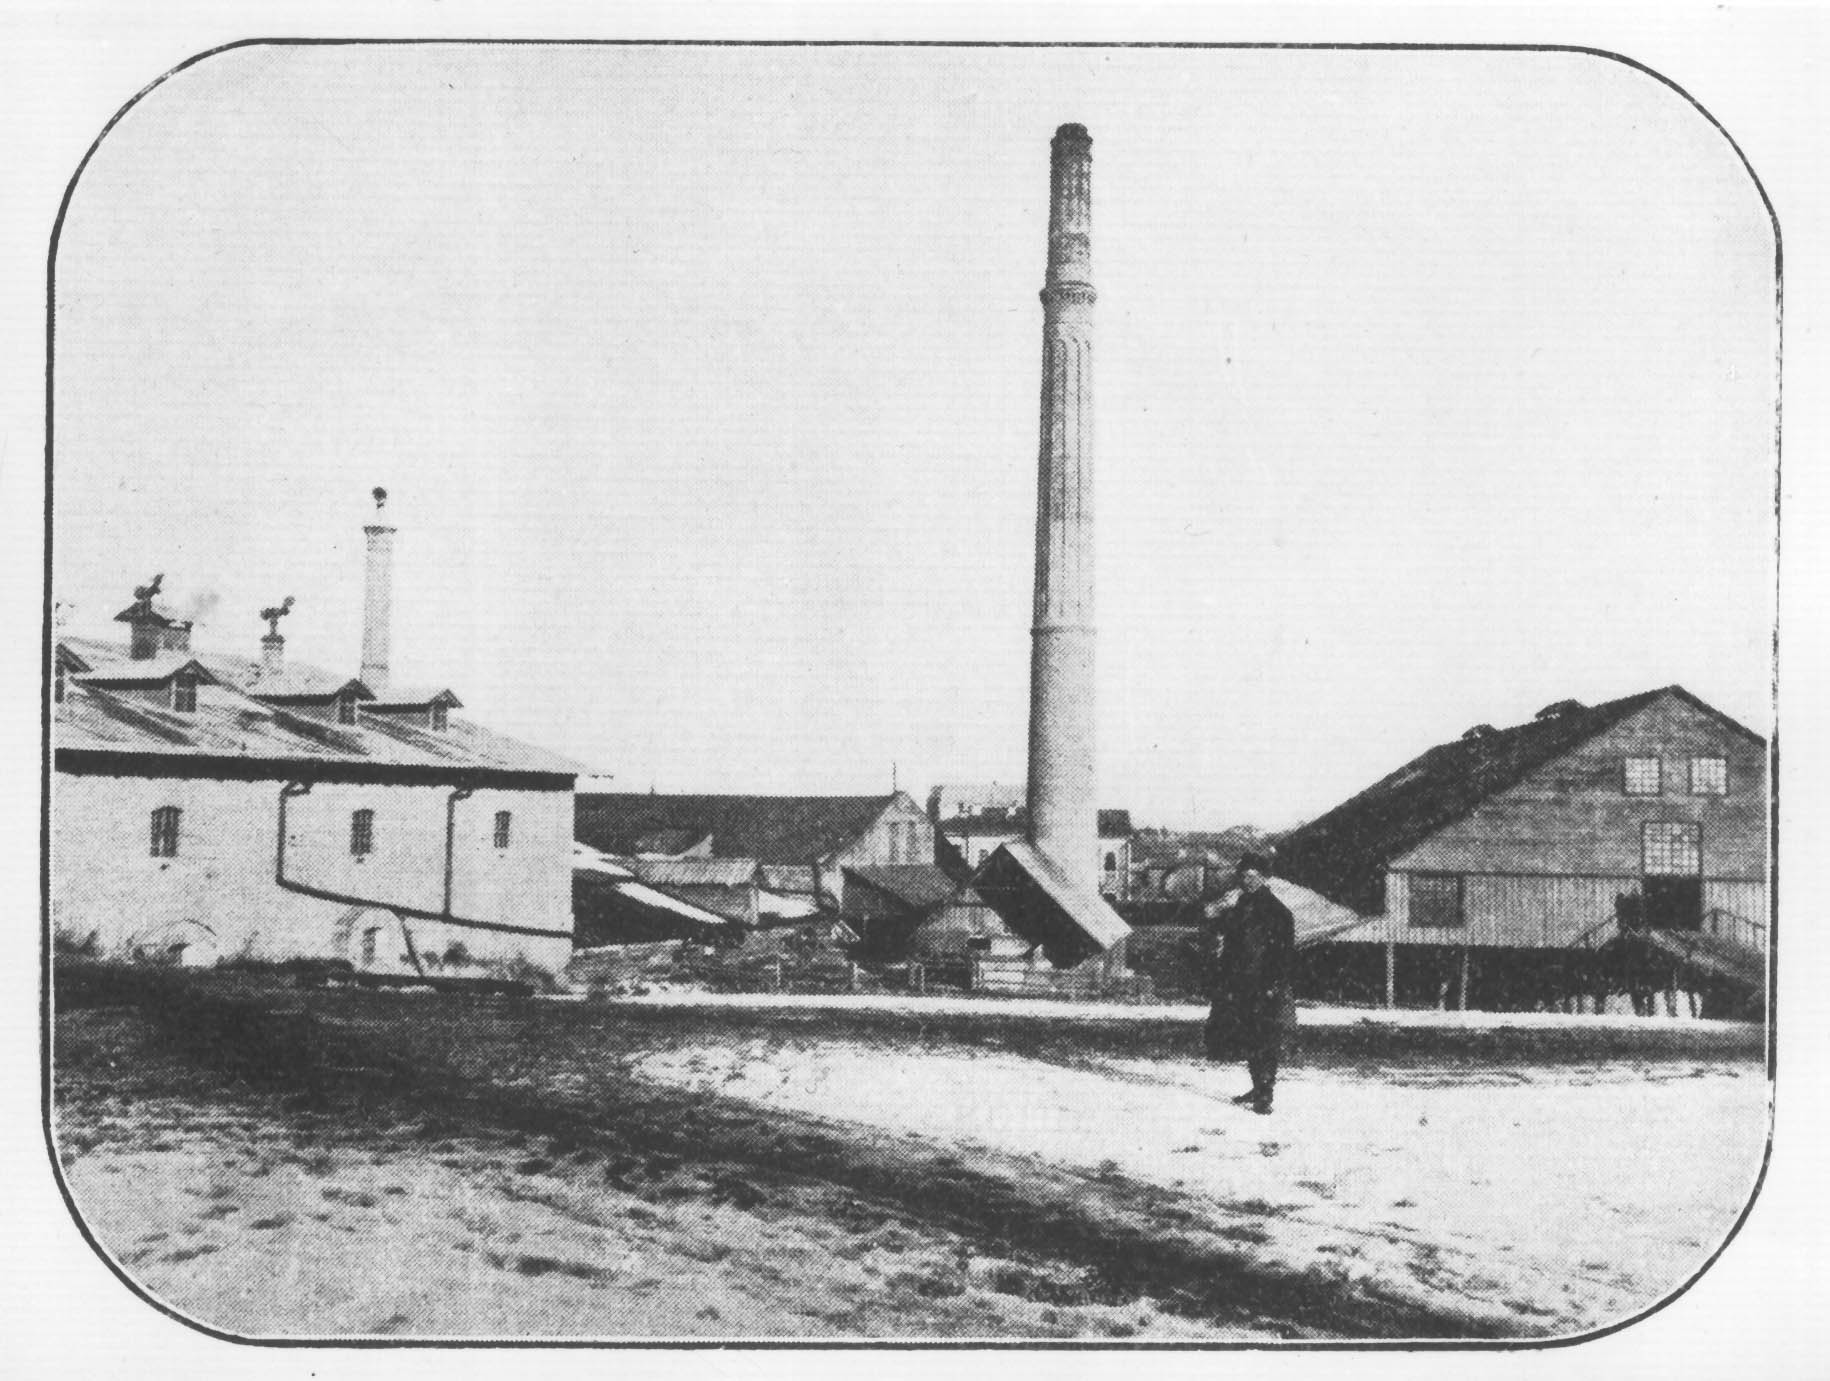
\includegraphics[width=\linewidth]{pix/1897-rihert-kirp.jpg}

\textit{1897. Завод Рихерта.}
\end{center} 
\vspace*{\fill}
\newpage
\vspace*{\fill}
\begin{center}
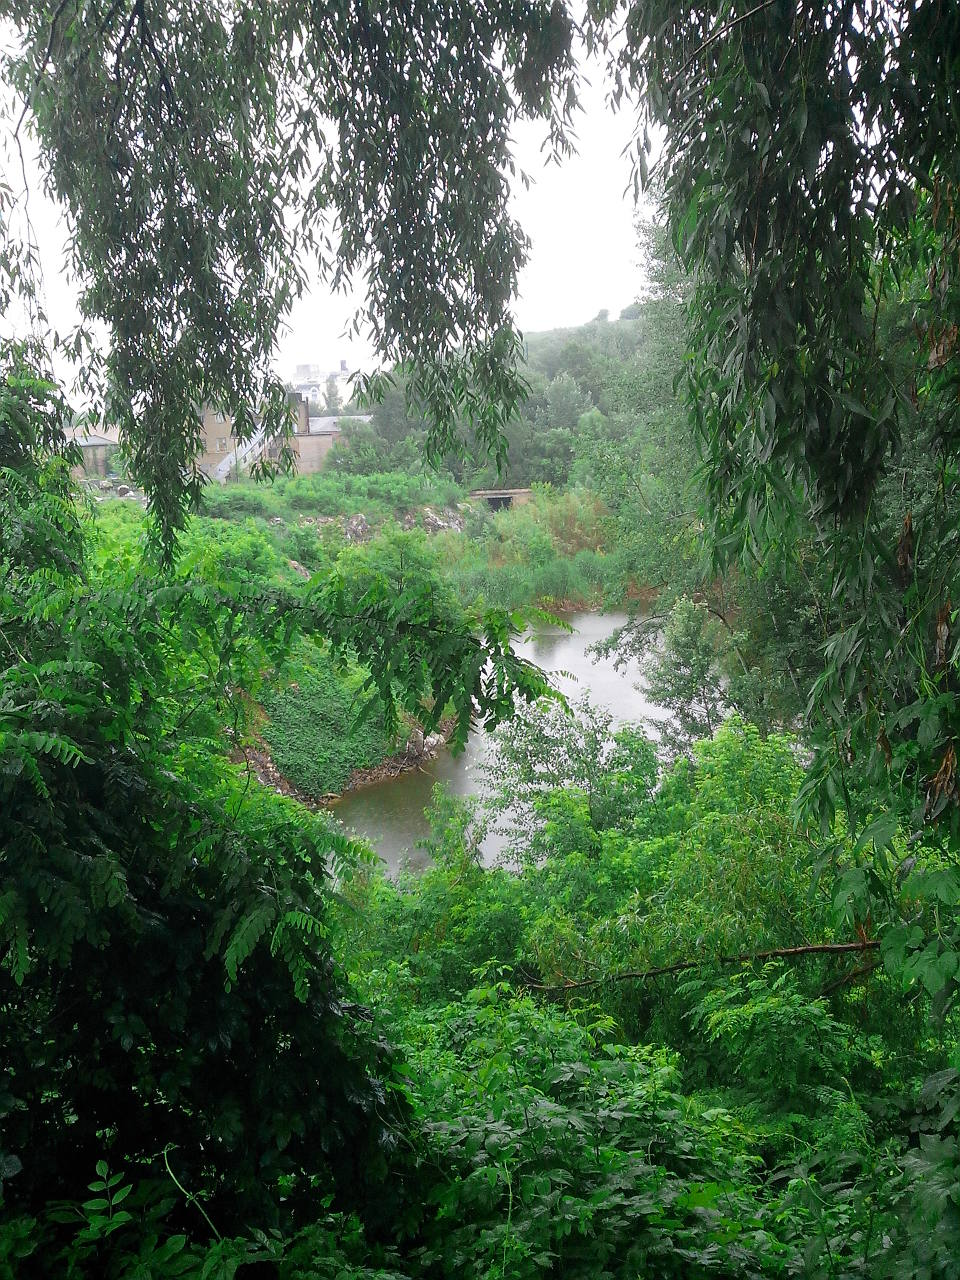
\includegraphics[width=\linewidth]{pix/s-rihert-IMG_20130602_161845.jpg}

\textit{2013. Карьерное озеро за бывшим заводом Рихерта.}
\end{center} 
\vspace*{\fill}
\newpage

\begin{center}
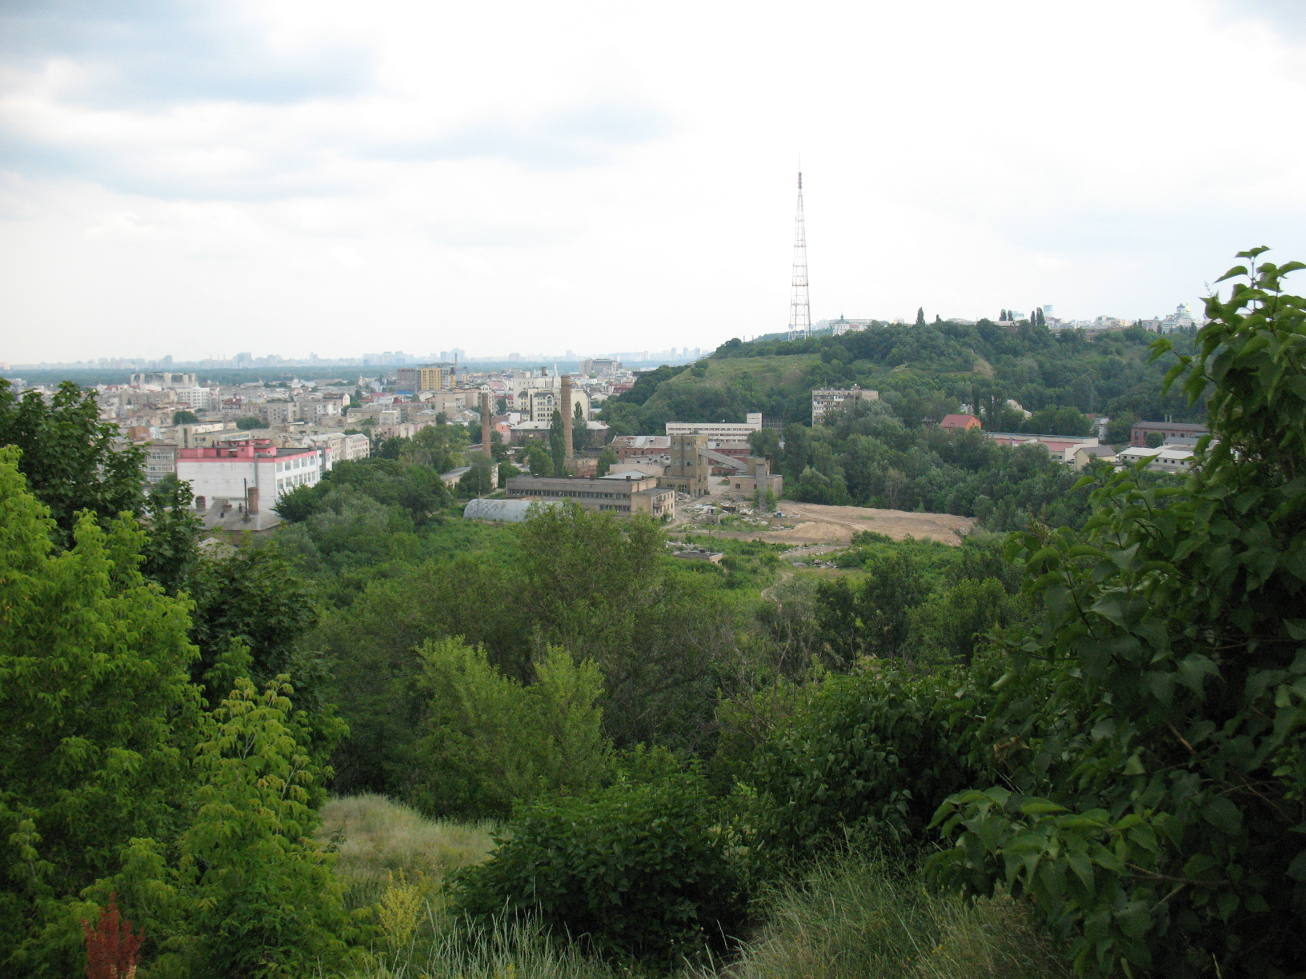
\includegraphics[width=0.98\linewidth]{pix/s-rihert-IMG_4358.JPG}

\textit{2015. Вид на бывший завод Рихерта с севера. На месте грязи раньше был склон Лысой горы.}
\end{center} 

\begin{center}
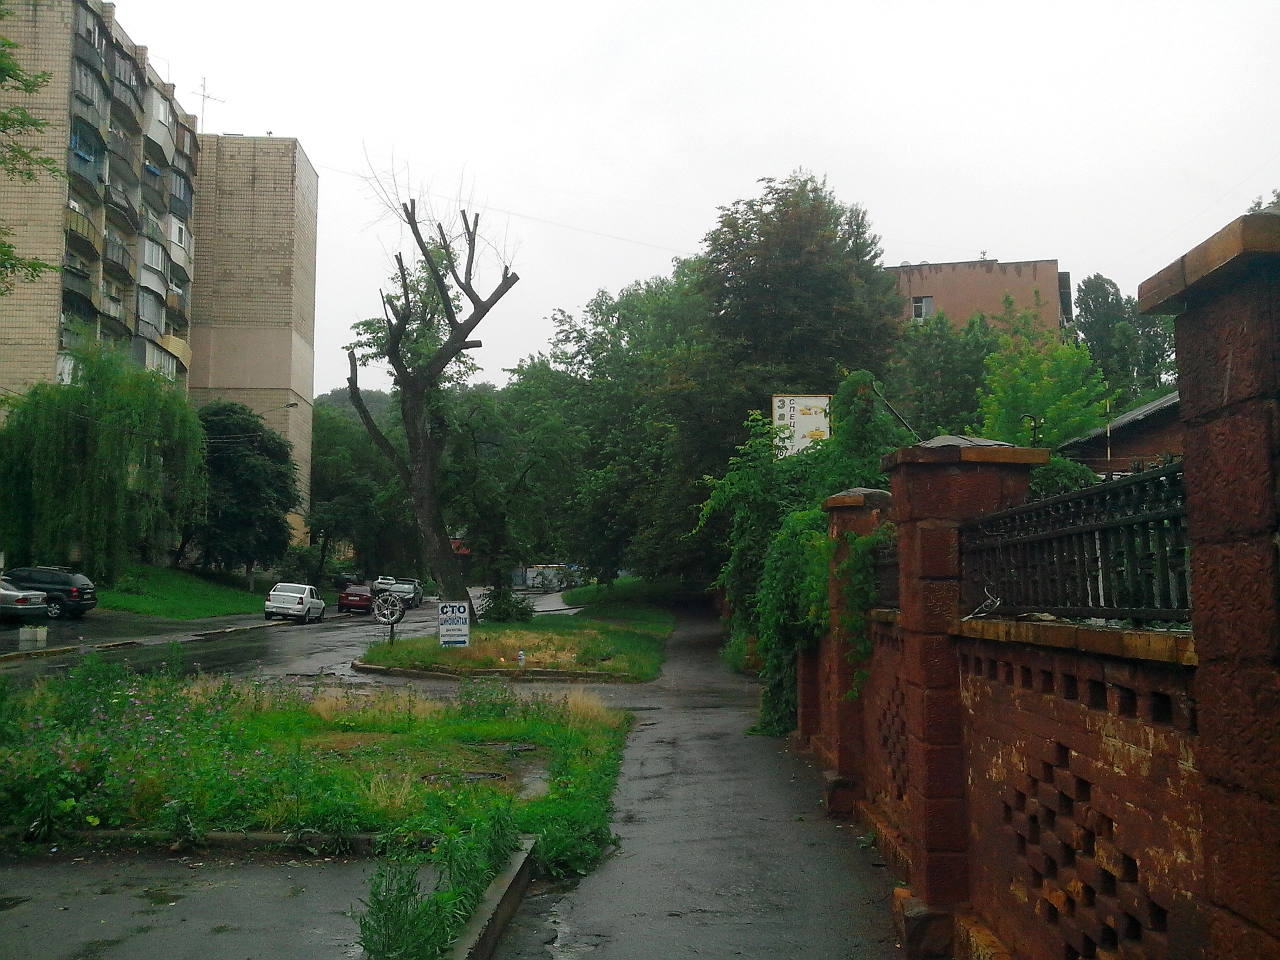
\includegraphics[width=0.98\linewidth]{pix/s-rihert-IMG_20130602_163103.jpg}

\textit{2013. Заводской забор на Нижнеюрковской, 2.}
\end{center} 

\newpage

\begin{center}
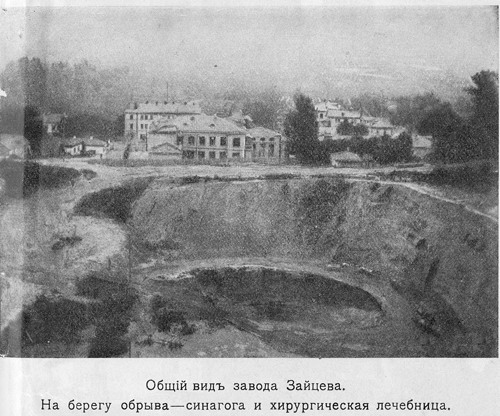
\includegraphics[width=\linewidth]{pix/zavod-zaiceva.png}
\end{center} 

\begin{center}
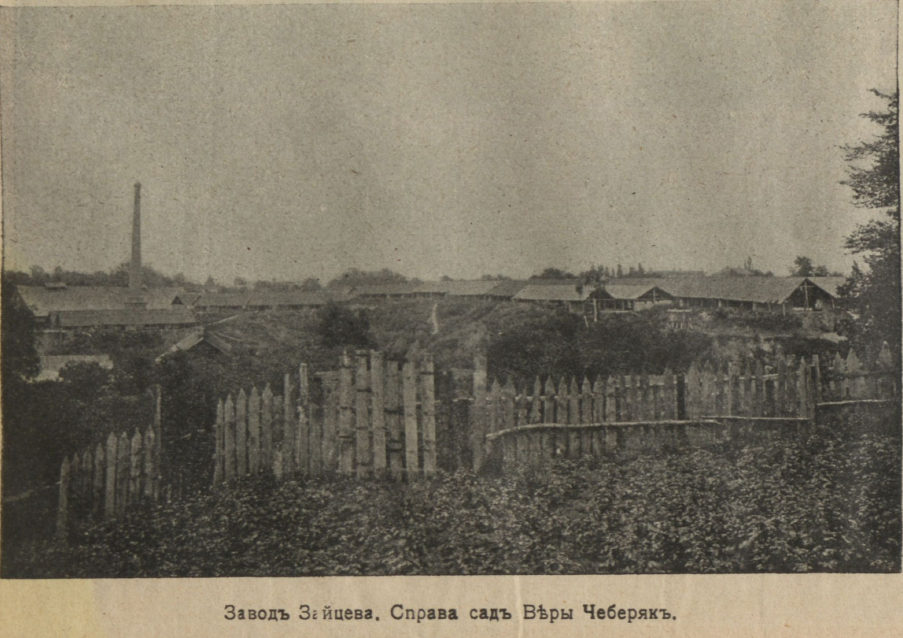
\includegraphics[width=\linewidth]{pix/1912-beylis-03.jpg}
\end{center} 

\newpage
\vspace*{\fill}
\begin{center}
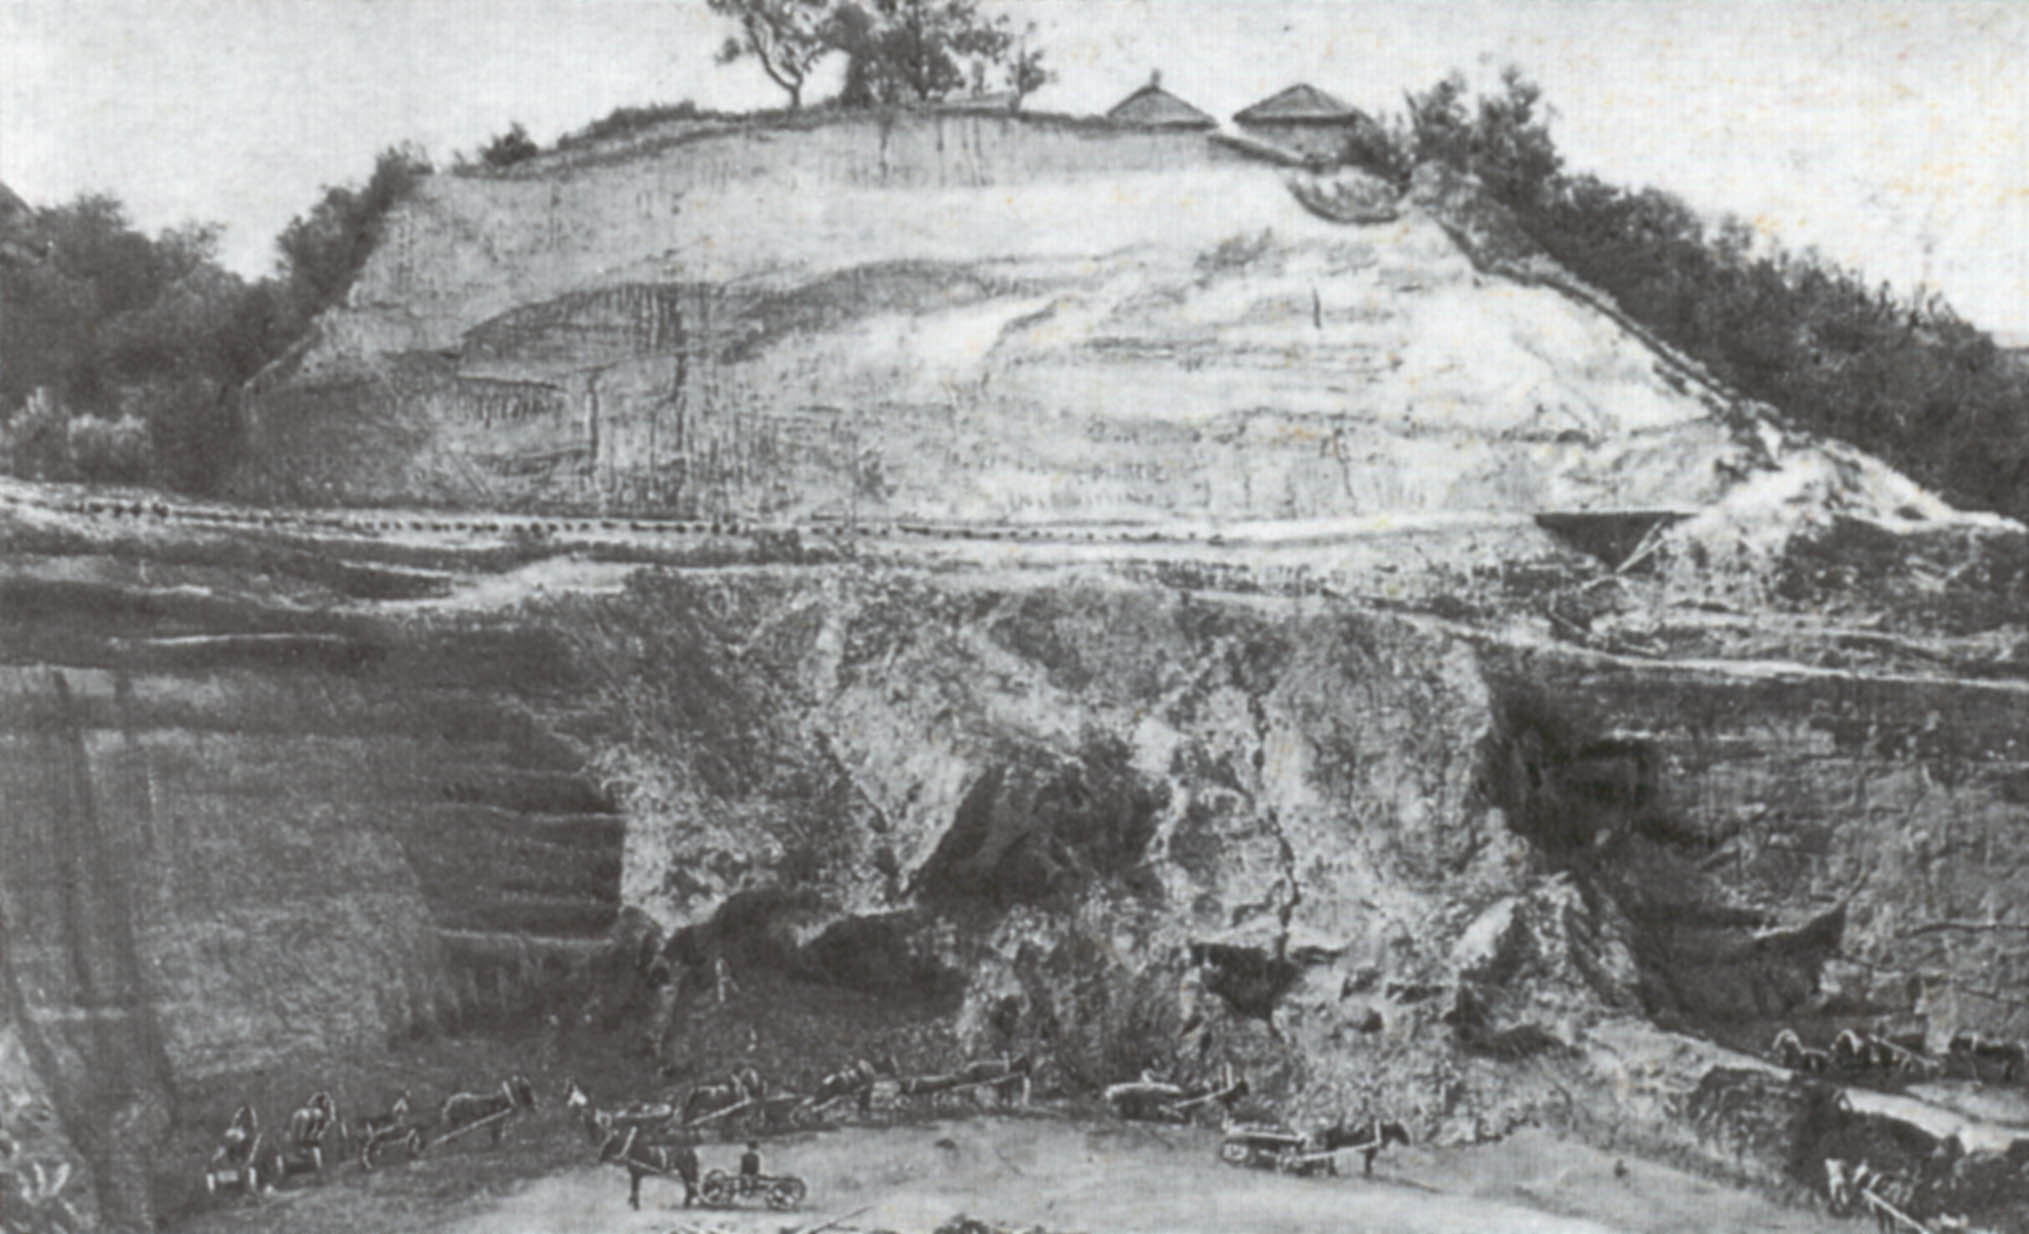
\includegraphics[width=\linewidth]{pix/hvoyka-02.jpg}

\textit{Глинище завода Зайцева во время раскопок Кирилловской стоянки.}
\end{center} 

\begin{center}
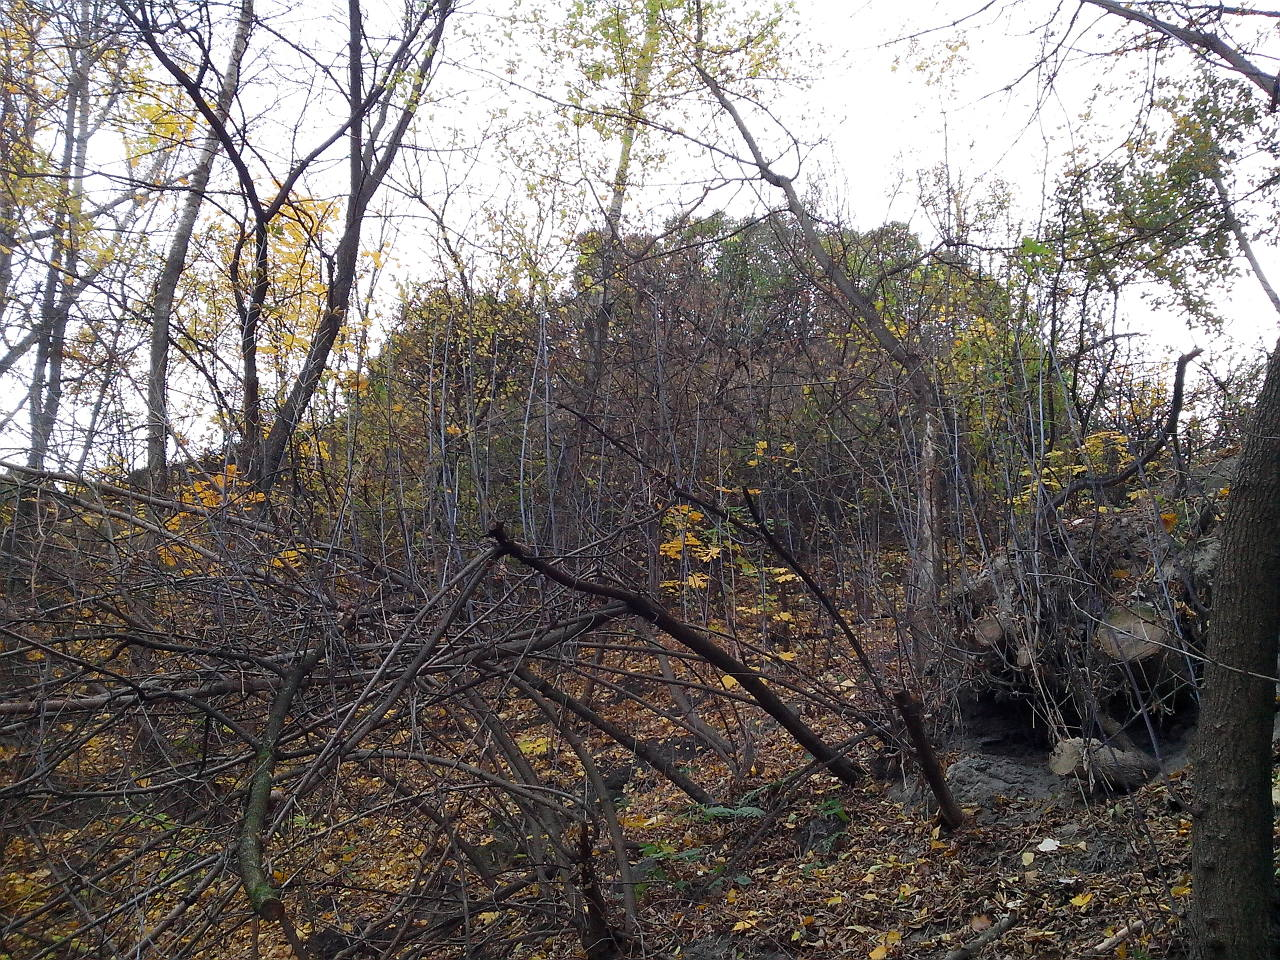
\includegraphics[width=\linewidth]{pix/s-IMG_20131020_163317.jpg}

\textit{2013. Остатки склона над глинищем.}
\end{center} 
\vspace*{\fill}
\newpage
\vspace*{\fill}
\begin{center}
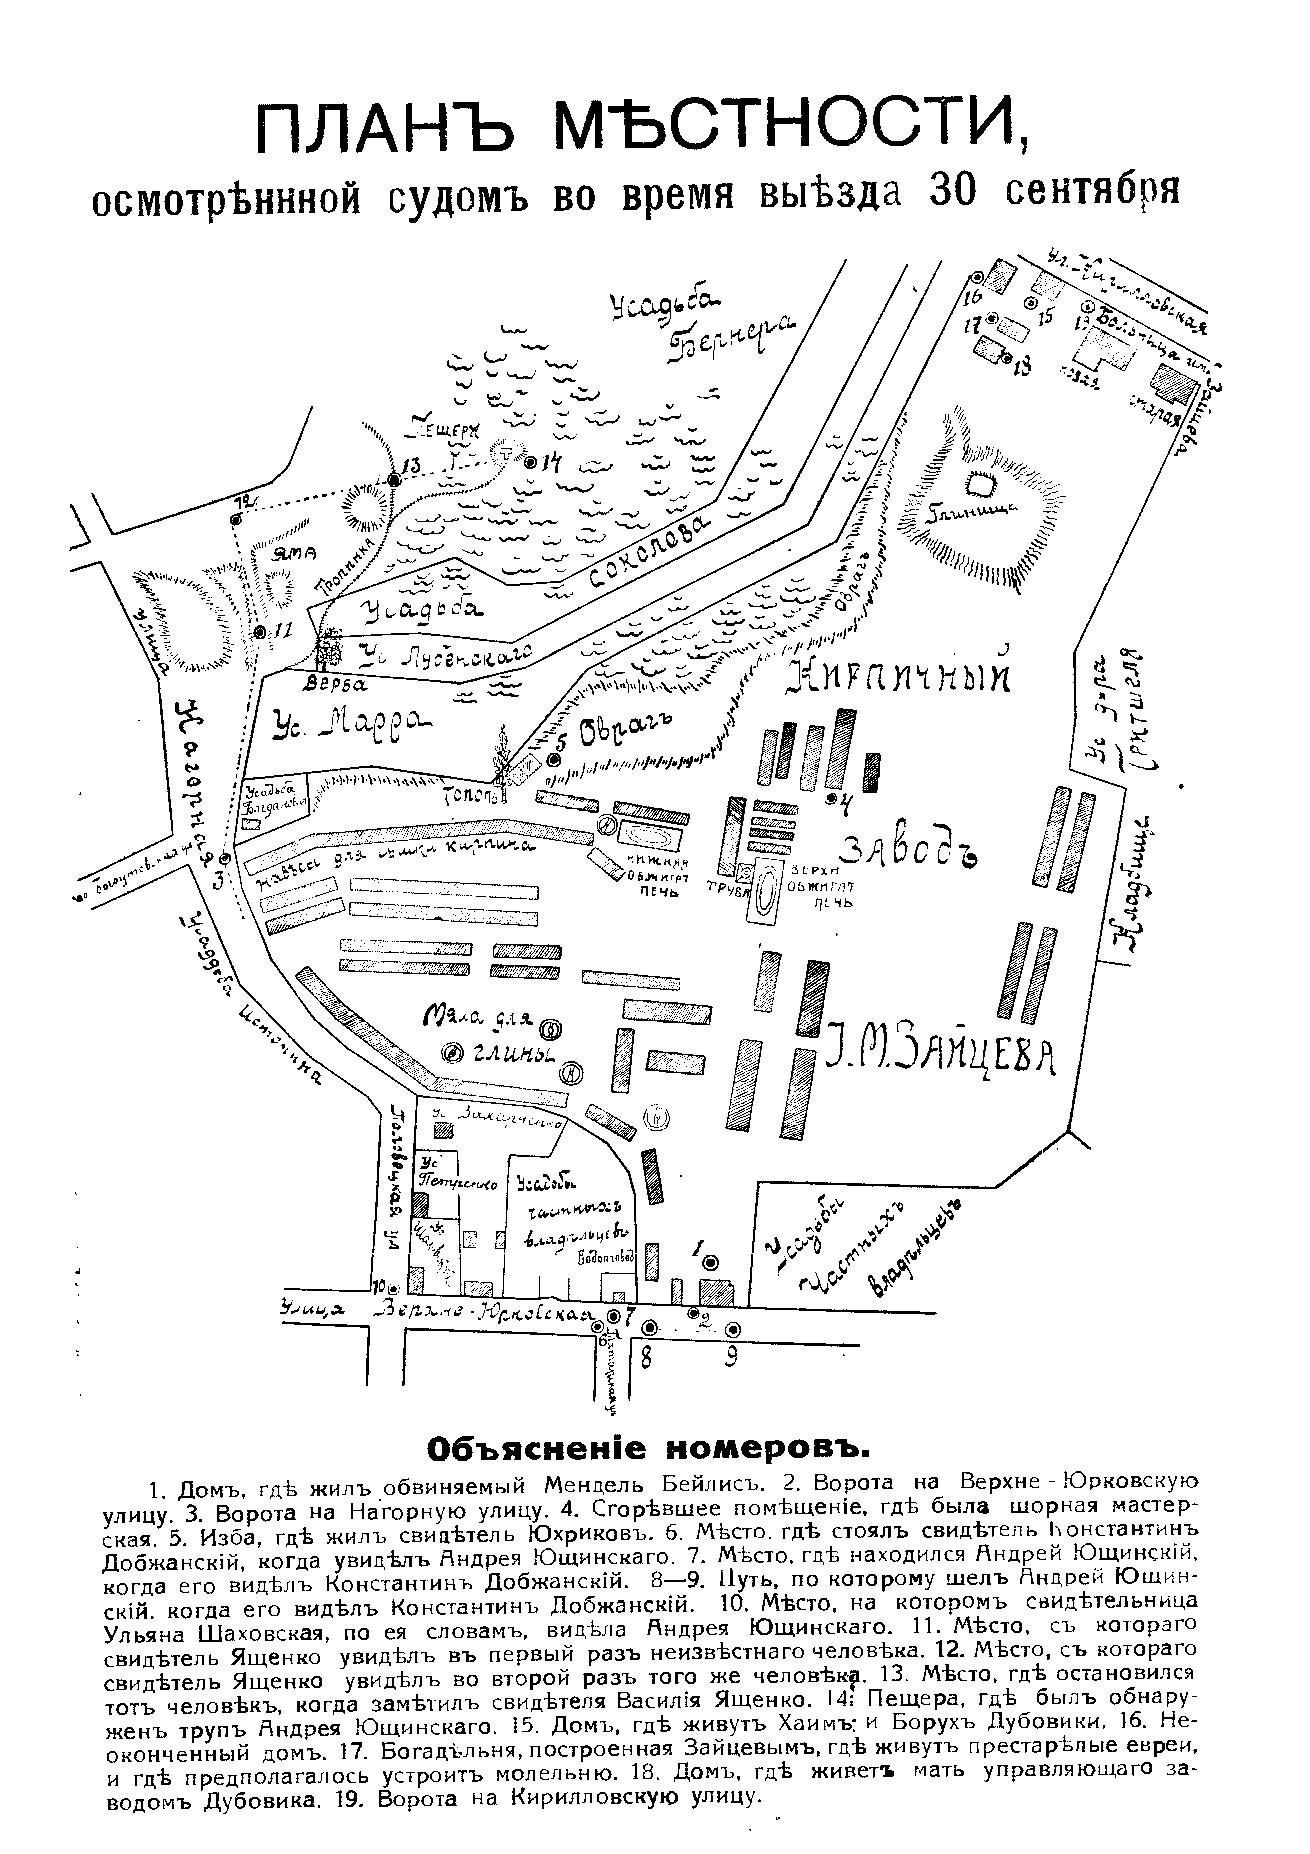
\includegraphics[width=\linewidth]{pix/1913-karta.jpg}

\textit{1913, карта из материалов дела Бейлиса.}
\end{center} 
\vspace*{\fill}
\newpage
\vspace*{\fill}
\begin{center}
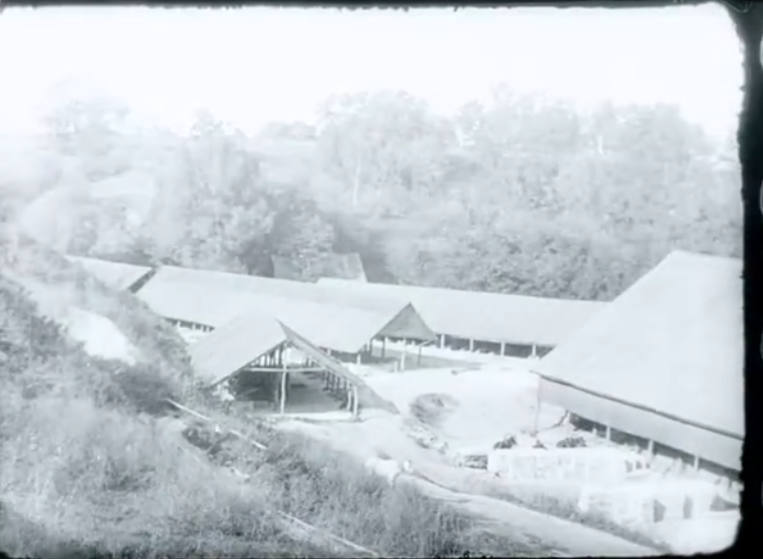
\includegraphics[width=\linewidth]{pix/zaic.jpg}
\end{center} 

\begin{center}
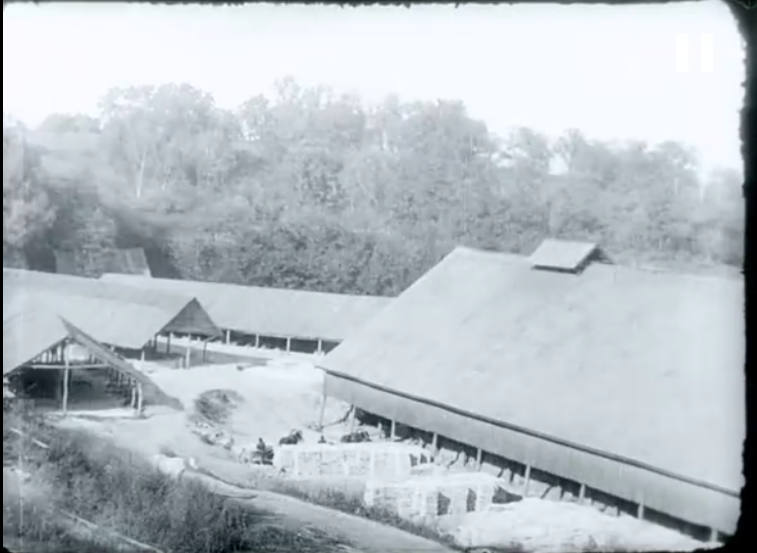
\includegraphics[width=\linewidth]{pix/zaic02.jpg}
\textit{1912. Кирпичный завод Зайцева вблизи.}
\end{center} 
\vspace*{\fill}
\newpage
\vspace*{\fill}
\begin{center}
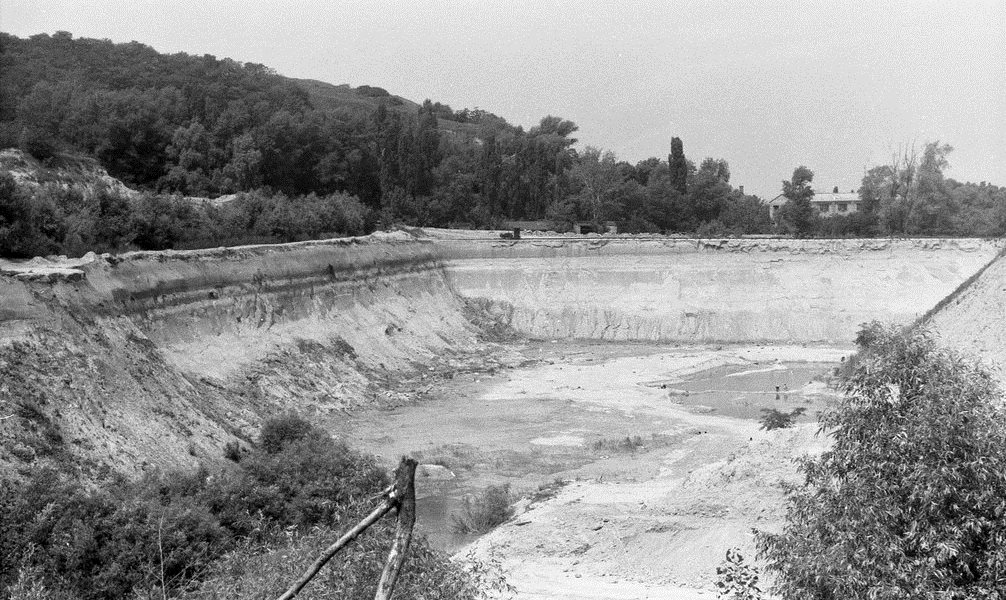
\includegraphics[width=\linewidth]{pix/syrec-06.jpg}

\textit{1950-60, один из карьеров Петровских кирпичных заводов в пойме речки Сырец.}
\end{center} 


\begin{center}
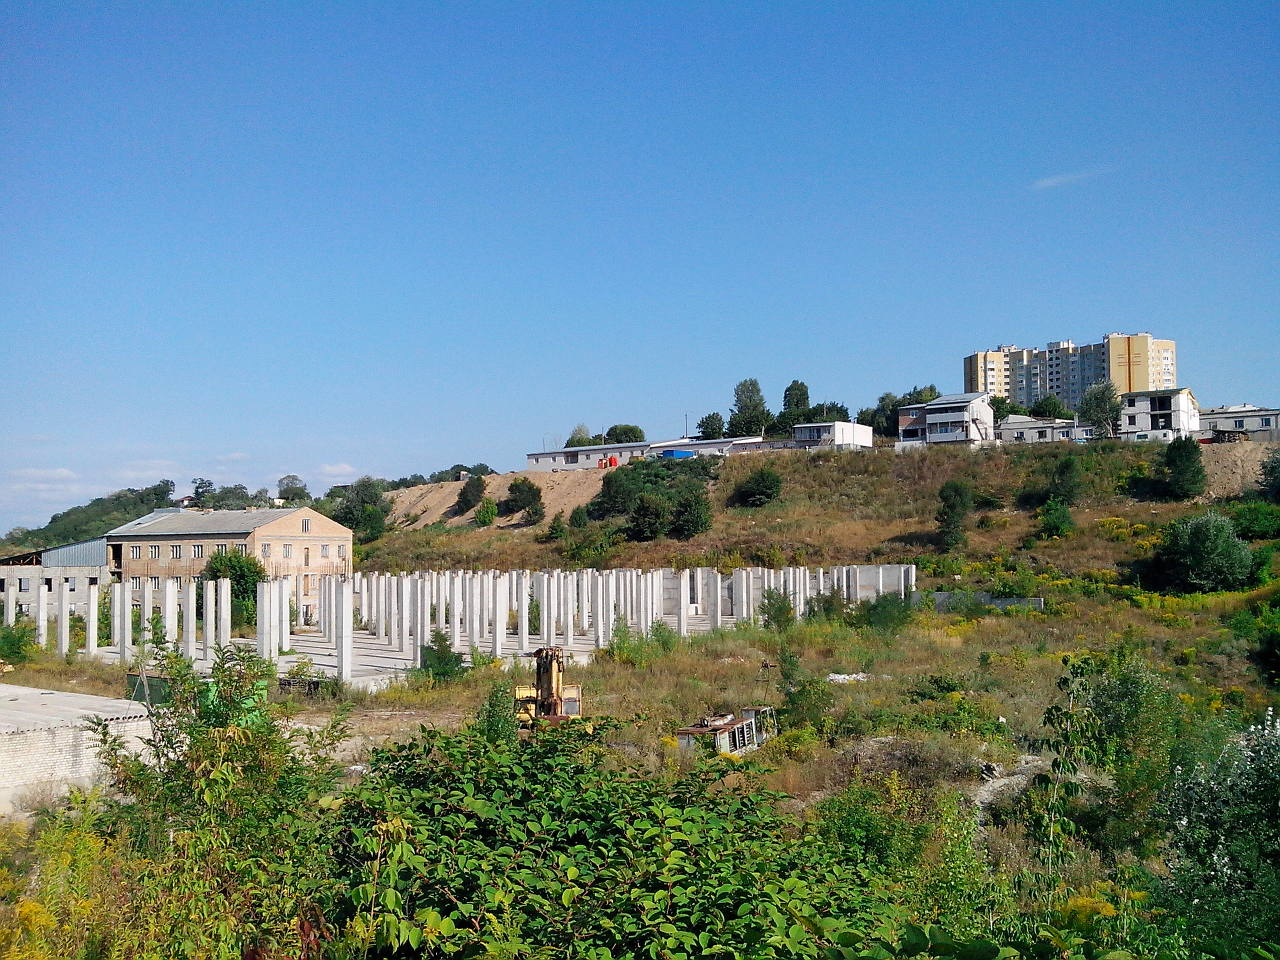
\includegraphics[width=\linewidth]{pix/s-syrec-IMG_20130812_163717.jpg}

\textit{2013, склоны глинища Петровских заводов за Сырецкой, 33Ш.}
\end{center} 
\vspace*{\fill}
\newpage

\begin{center}
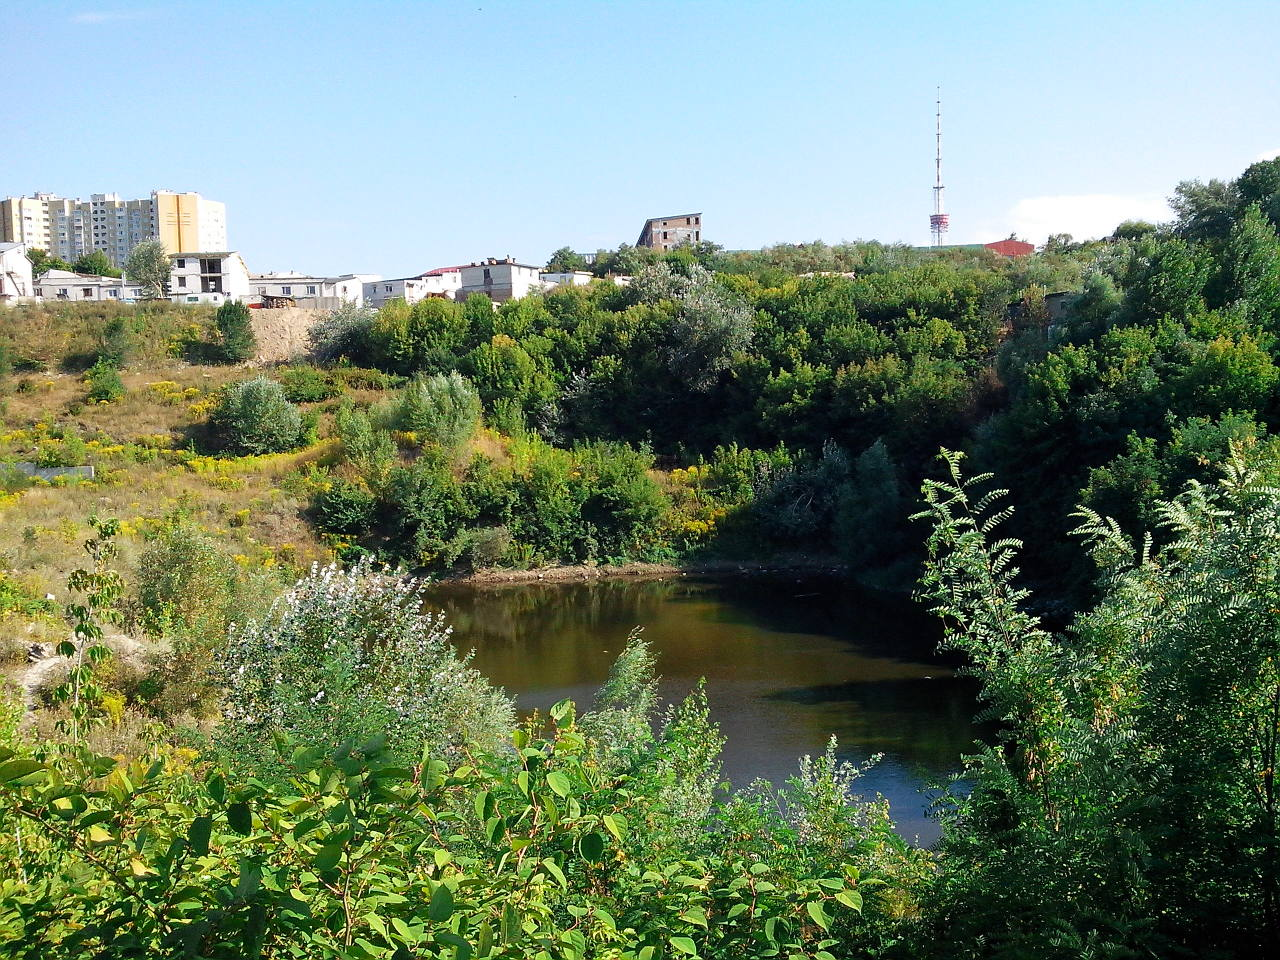
\includegraphics[width=\linewidth]{pix/s-syrec-IMG_20130812_163712.jpg}

\textit{2013, там же, карьерное озеро.}
\end{center} 

\begin{center}
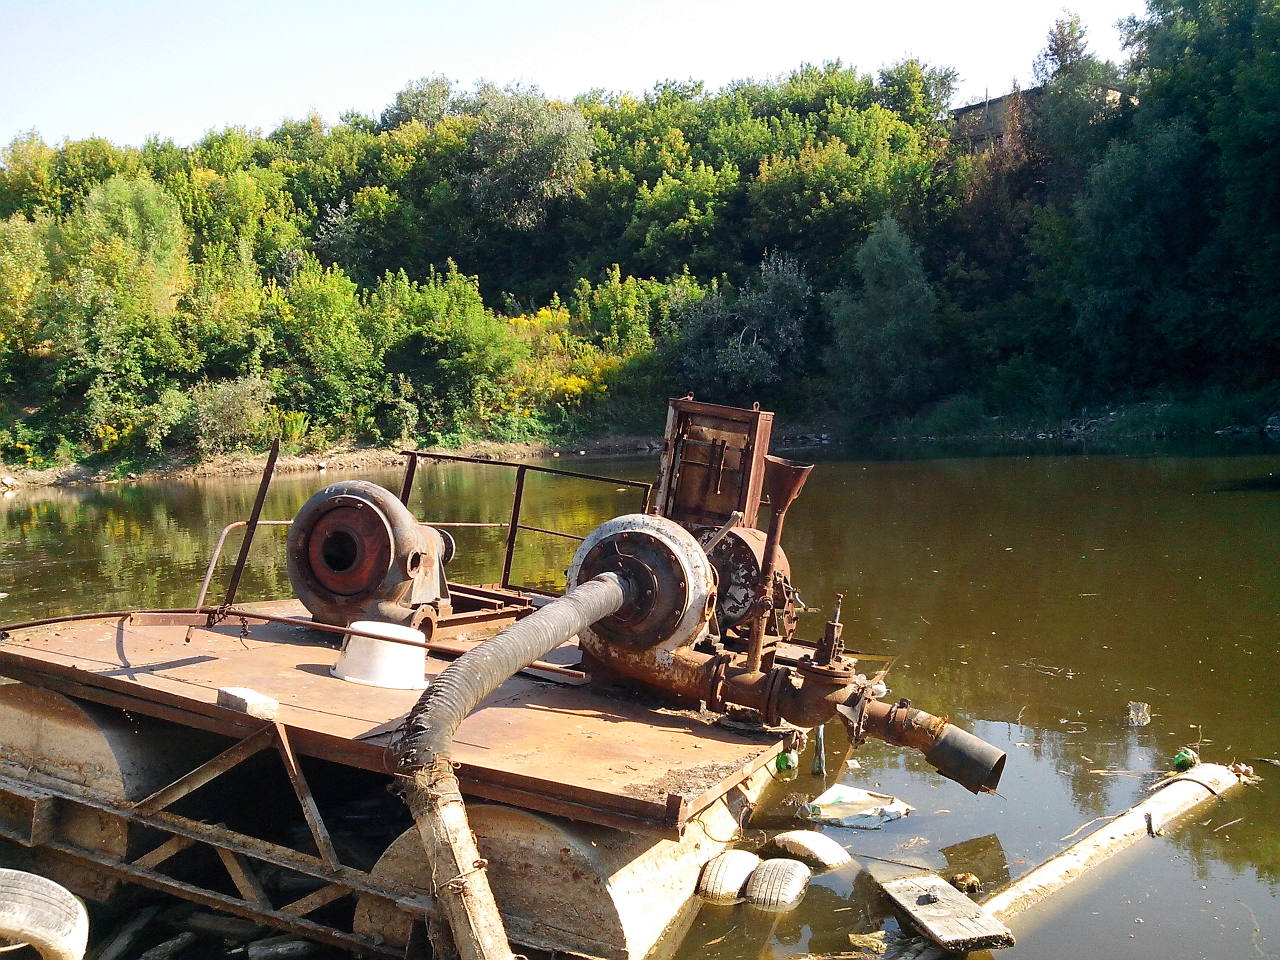
\includegraphics[width=\linewidth]{pix/s-syrec-IMG_20130812_164051.jpg}

\textit{2013, там же.}
\end{center} 

\newpage
\vspace*{\fill}
\begin{center}
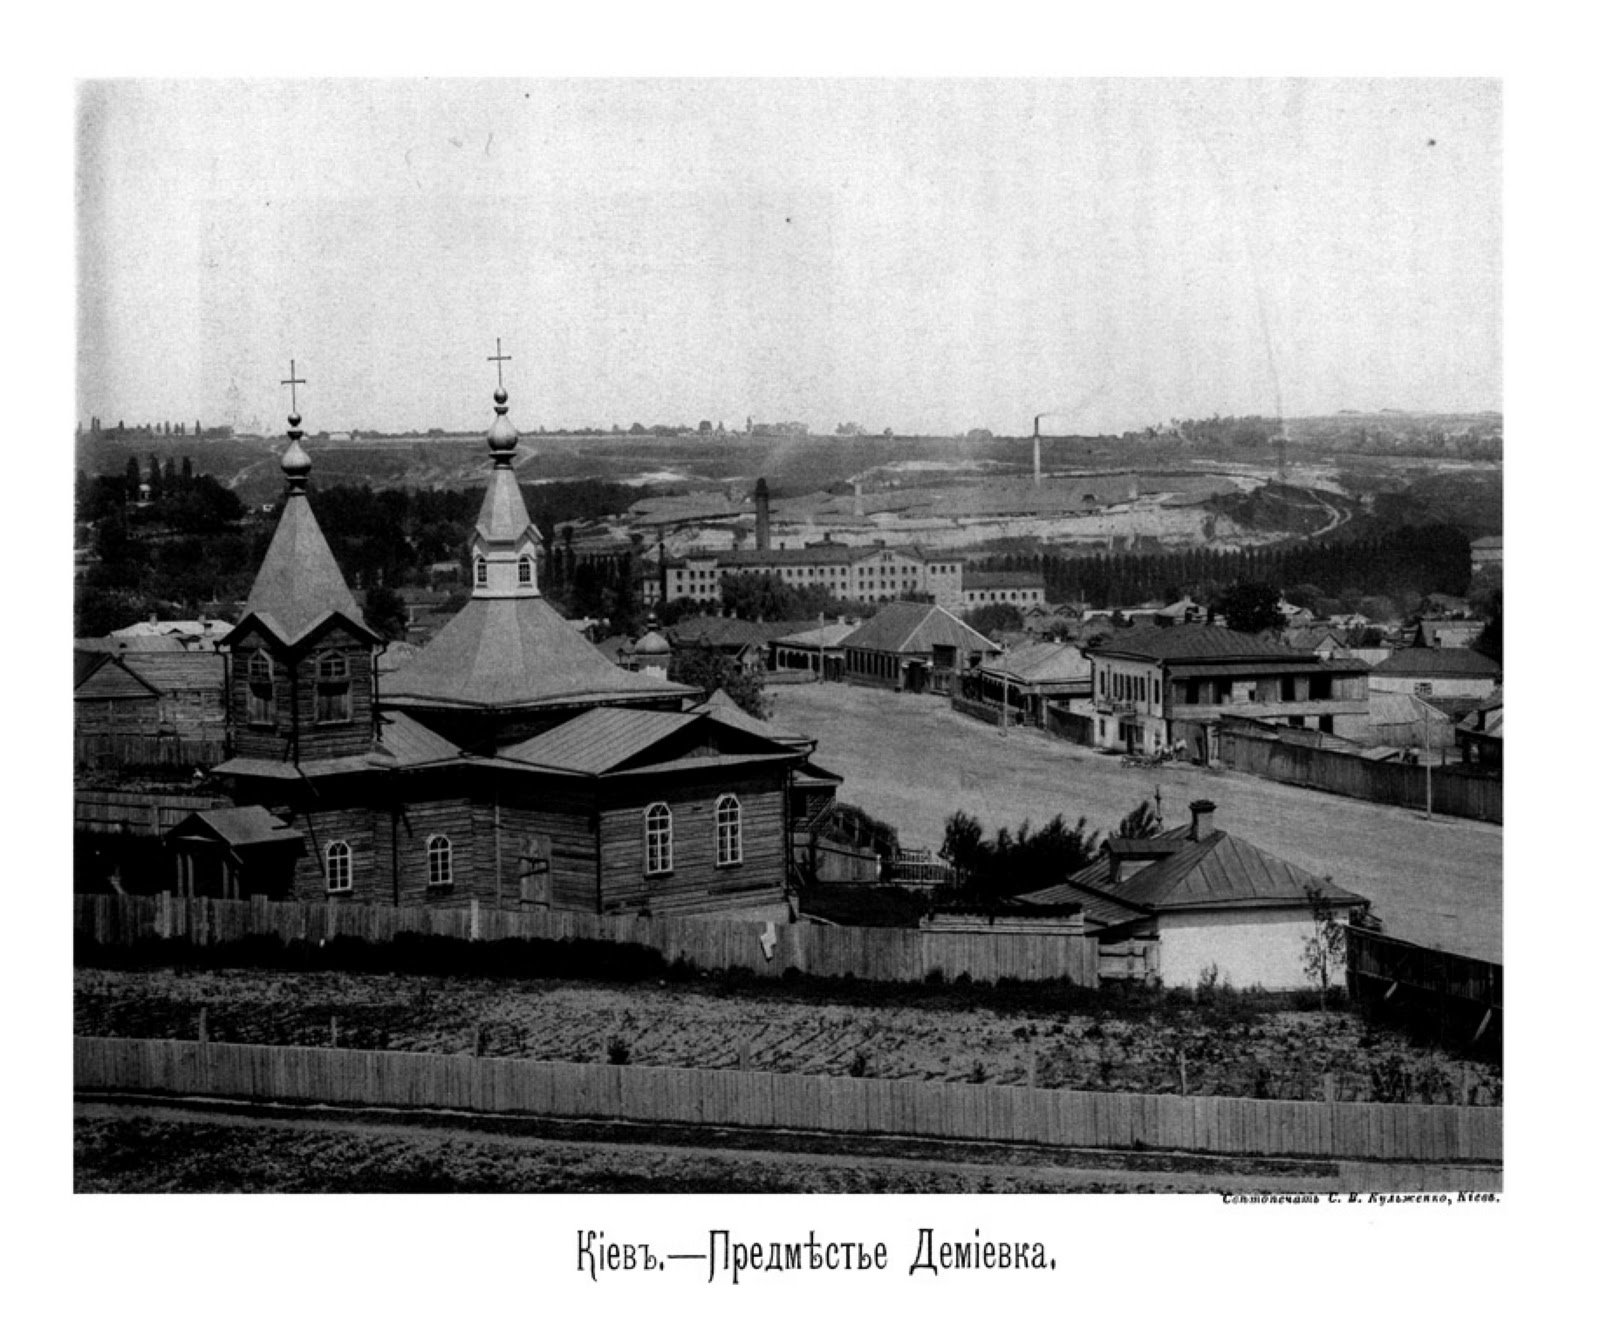
\includegraphics[width=\linewidth]{pix/24.jpeg}
\end{center} 

\textit{1888 год, фото из книги М. Захарченко «Киев теперь и прежде». Ближайшая труба на заднем плане – сахарорафинадного завода (в советское время там расположилась кондитерская фабрика имени Карла Маркса), а вот за ним – трубы заводов Субботиной и Шатовой, и глинища оных. Слева – Вознесенская церковь, стоит и поныне, на Голосеевском проспекте.}
\vspace*{\fill}
\newpage
\vspace*{\fill}
\begin{center}
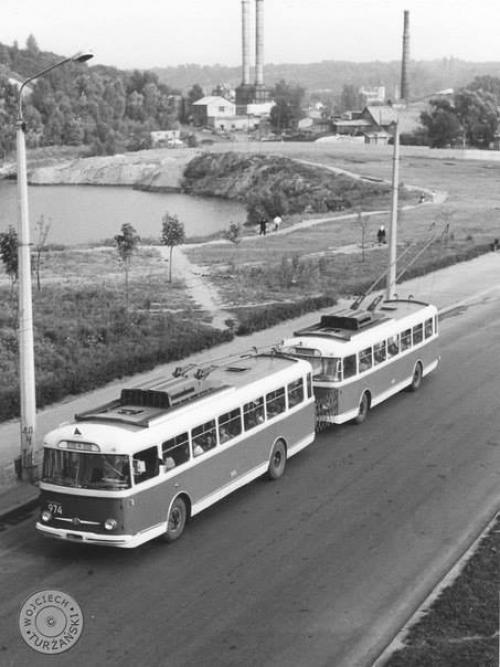
\includegraphics[width=\linewidth]{pix/woitech.jpg}
\end{center} 

\textit{После 1966 года, озеро Глинка (частично по месту глинища Субботиной), на заднем плане – трубы кирпичного завода. Фото Wojtiech Turzanski.}
\vspace*{\fill}
\newpage

\begin{center}
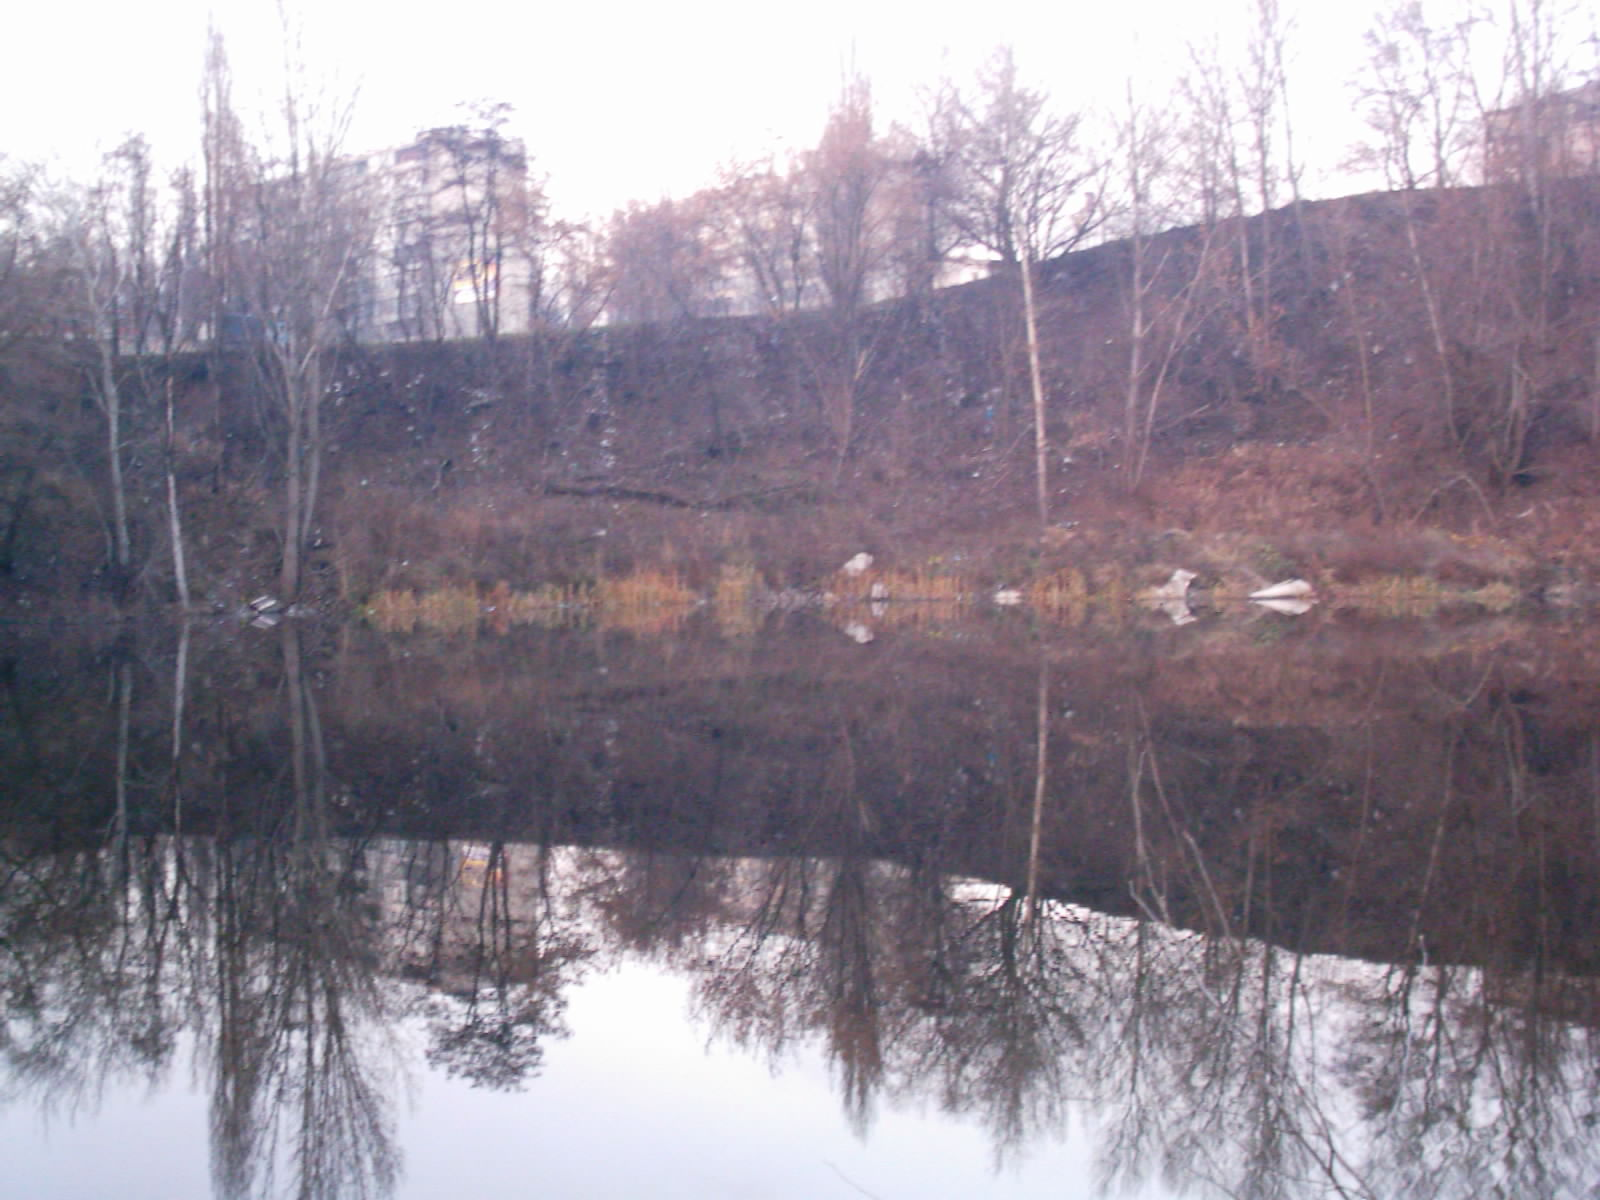
\includegraphics[width=\linewidth]{pix/glinka-imag0022.jpg}
\textit{2005, озеро Глинка.}
\end{center} 

\begin{center}
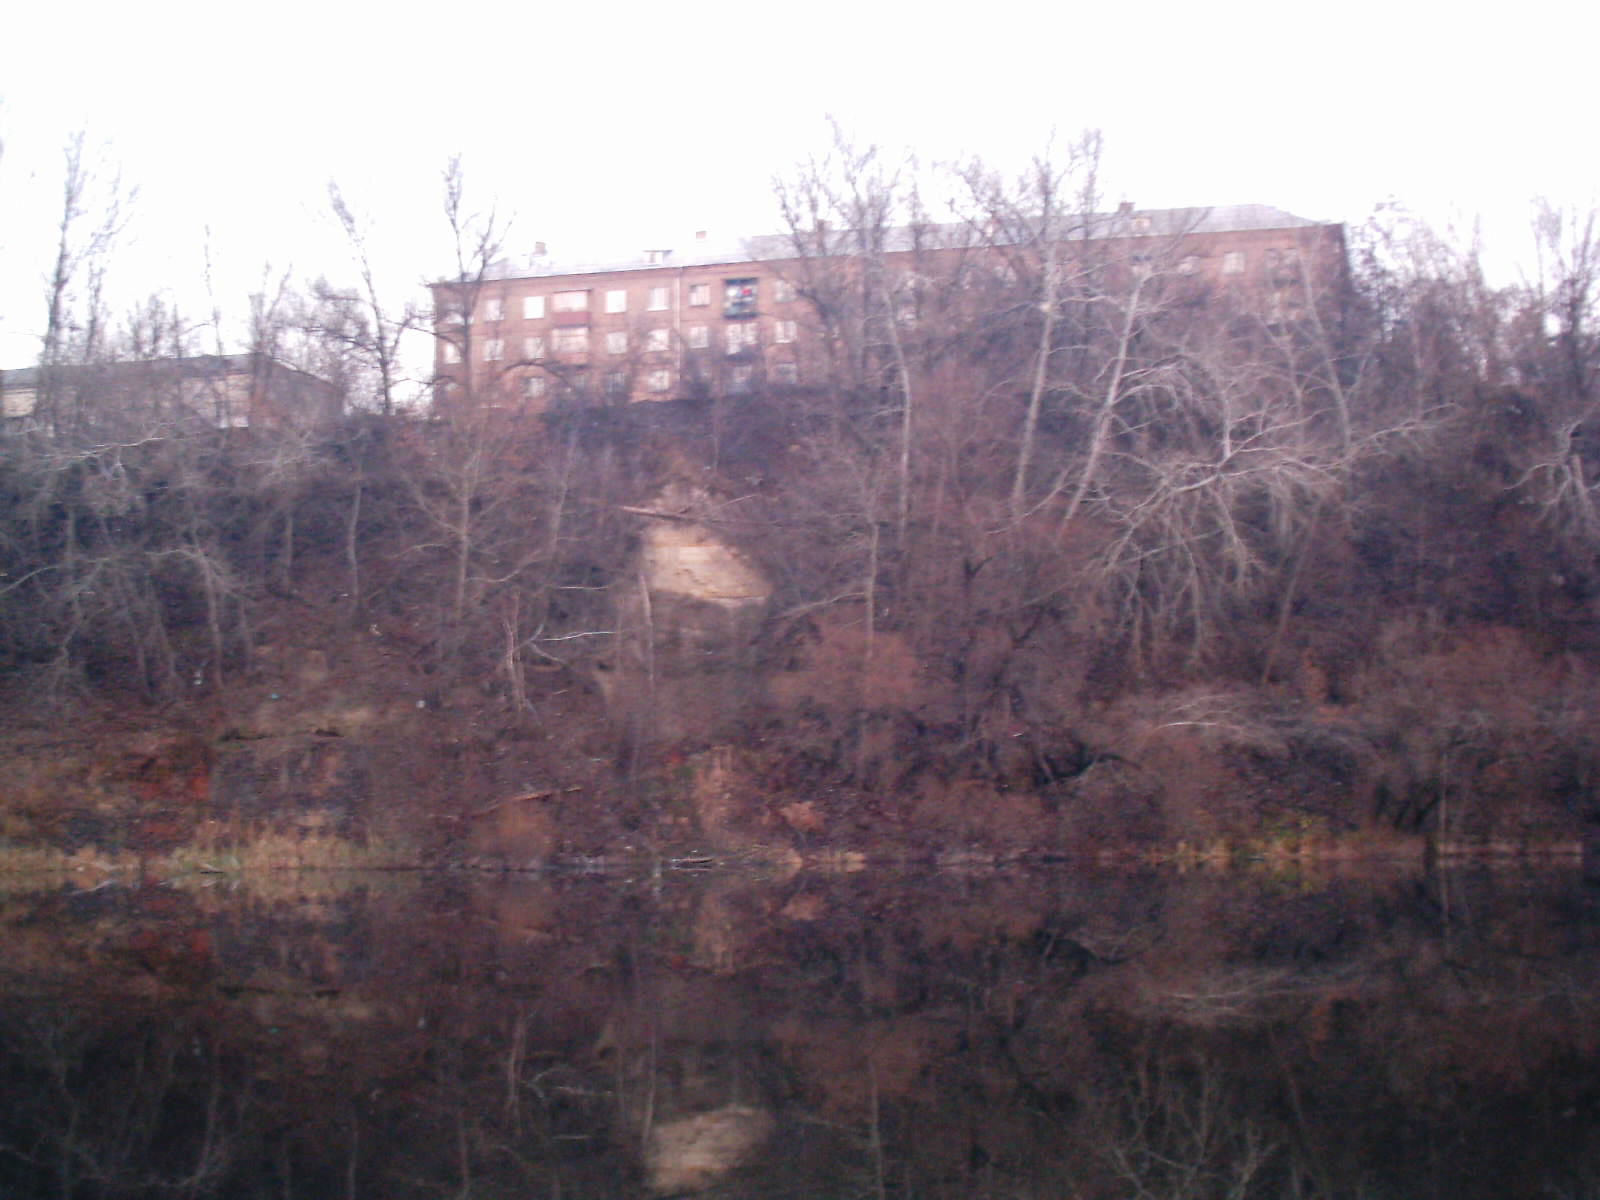
\includegraphics[width=\linewidth]{pix/glinka-imag0018.jpg}

\textit{2005, озеро Глинка.}
\end{center} 
\newpage

\begin{center}
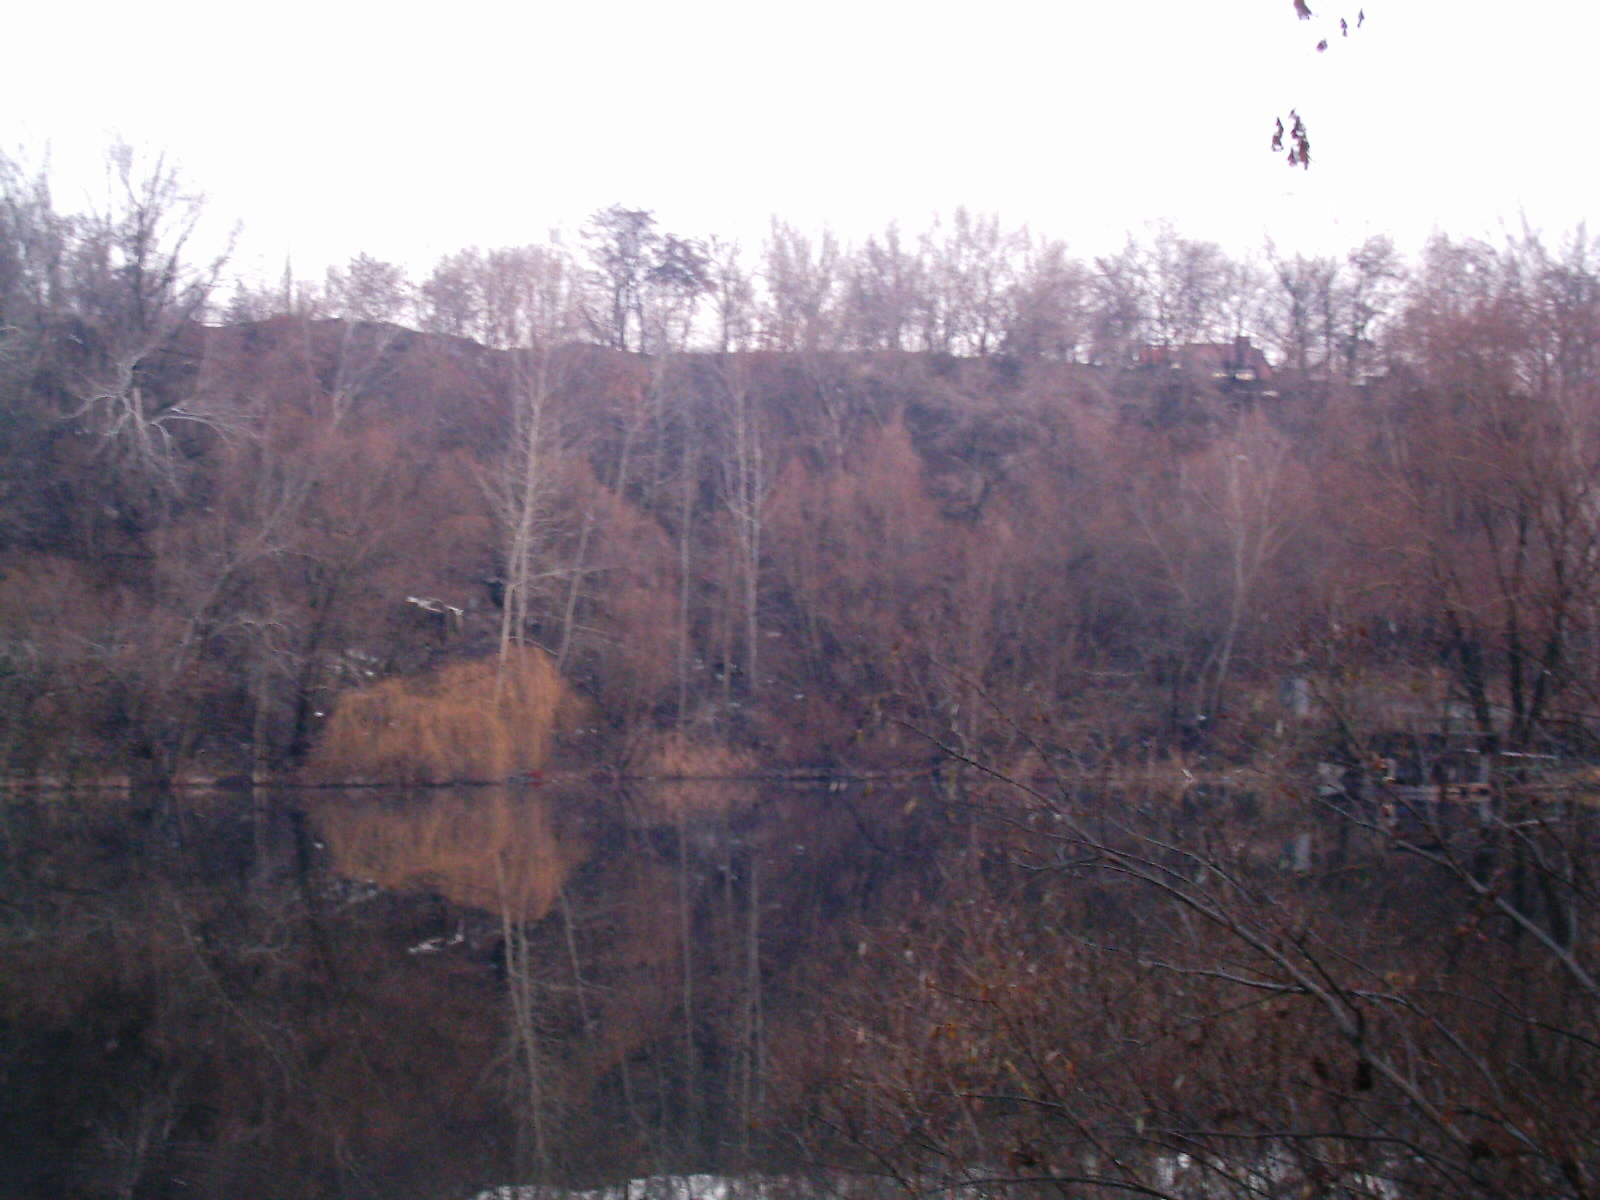
\includegraphics[width=\linewidth]{pix/glinka-imag0019.jpg}
\textit{2005, озеро Глинка.}
\end{center} 

\begin{center}
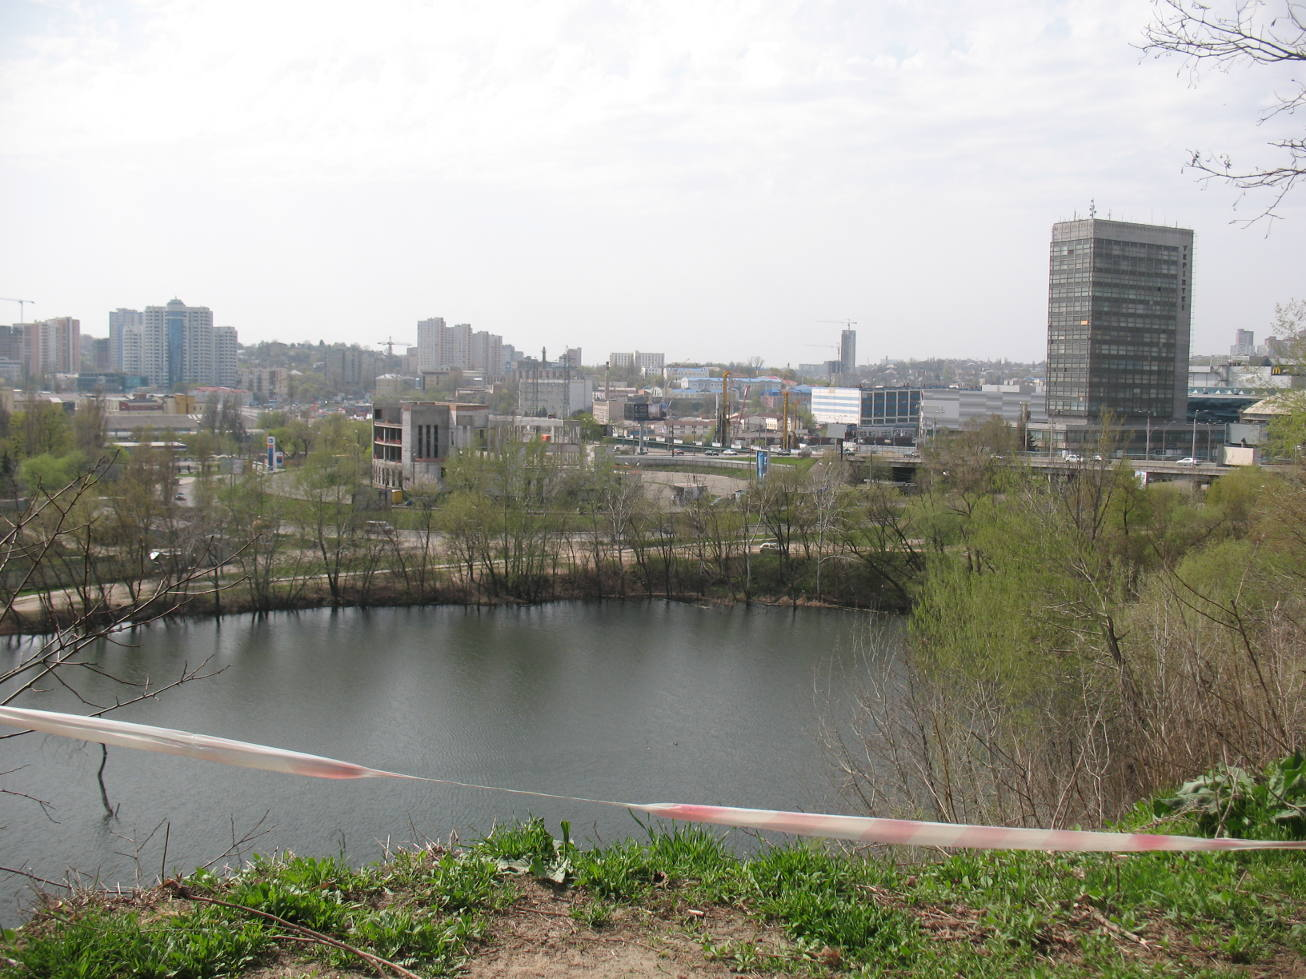
\includegraphics[width=\linewidth]{pix/s-glinka-IMG_4542.JPG}
\textit{2016, озеро Глинка, вид с обрыва. Позади – Демиевка.}
\end{center} 

\newpage

\begin{center}
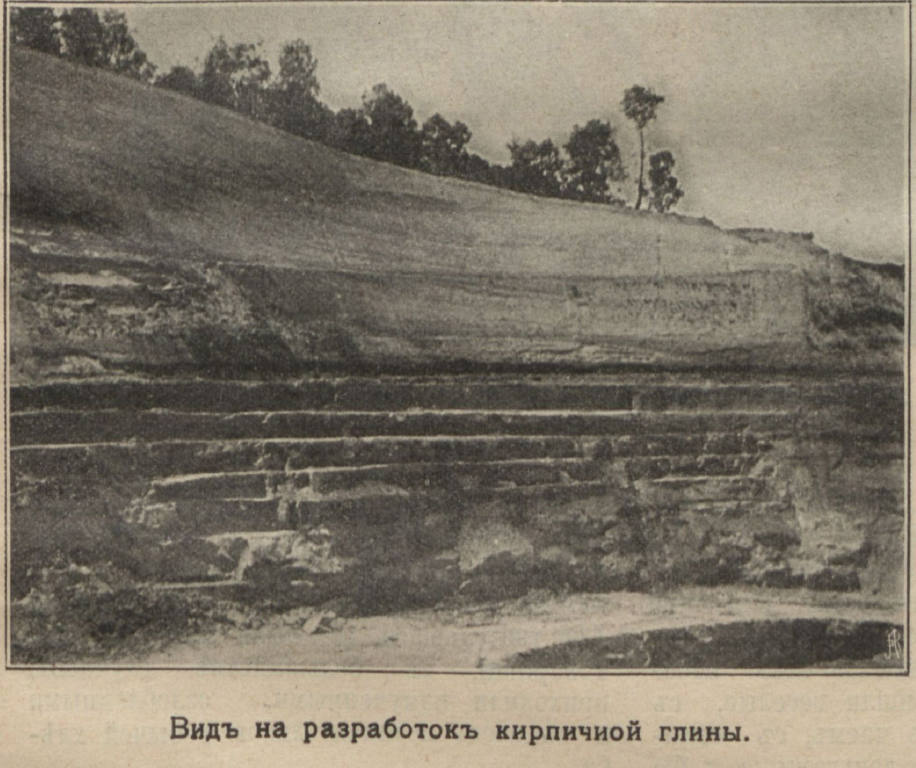
\includegraphics[width=0.91\linewidth]{pix/1910-01.jpg}
\end{center} 


\begin{center}
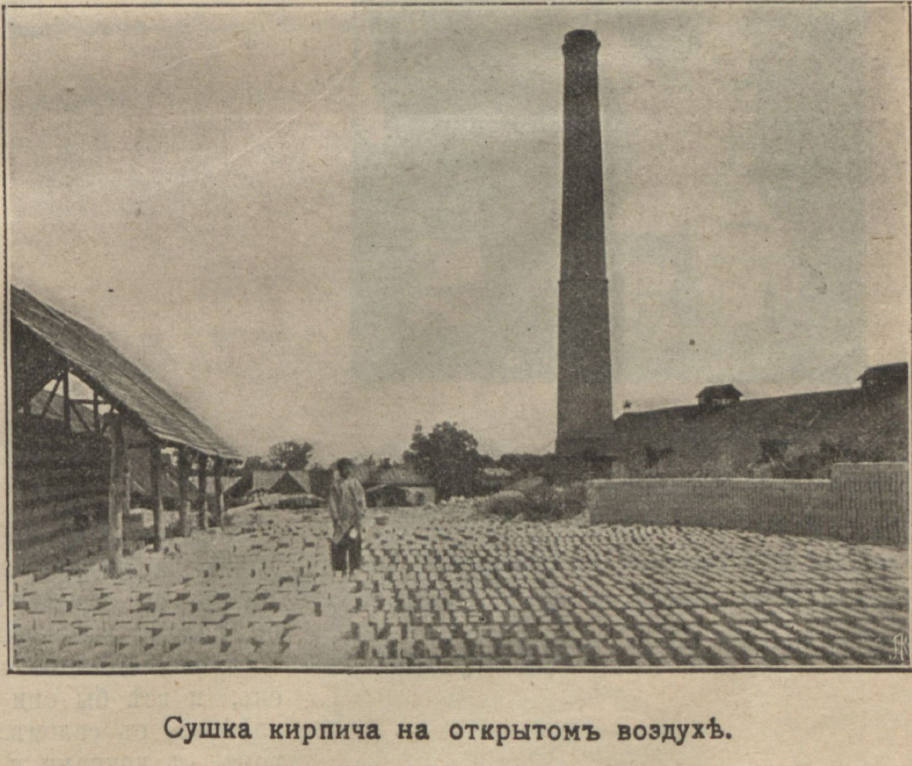
\includegraphics[width=0.91\linewidth]{pix/1910-02.jpg}

\textit{1910, фото из приложения к газете «Киевская мысль».}
\end{center} 

\newpage

\begin{center}
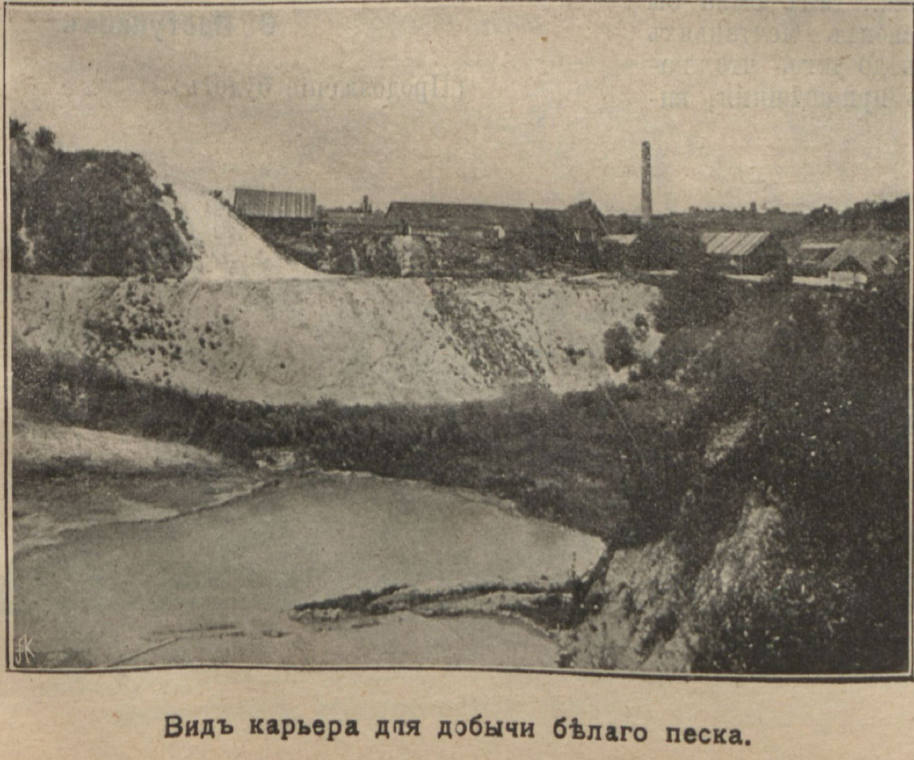
\includegraphics[width=0.91\linewidth]{pix/1910-03.jpg}
\end{center} 


\begin{center}
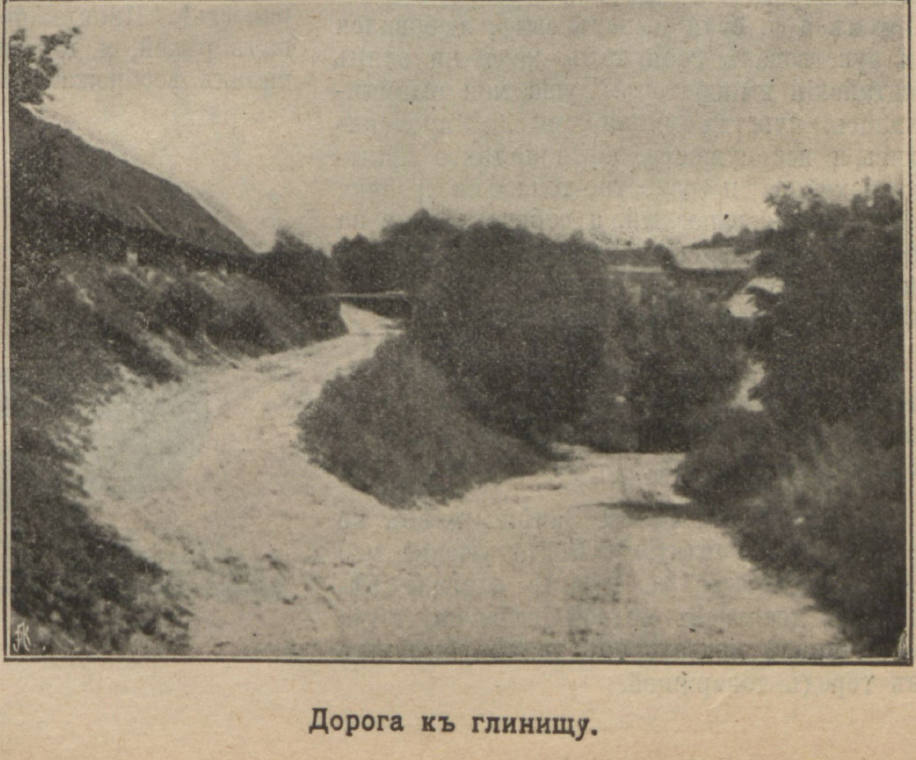
\includegraphics[width=0.91\linewidth]{pix/1910-04.jpg}

\textit{1910, фото из приложения к газете «Киевская мысль».}
\end{center} 

%\newpage
%\vspace*{\fill}
%\begin{center}
%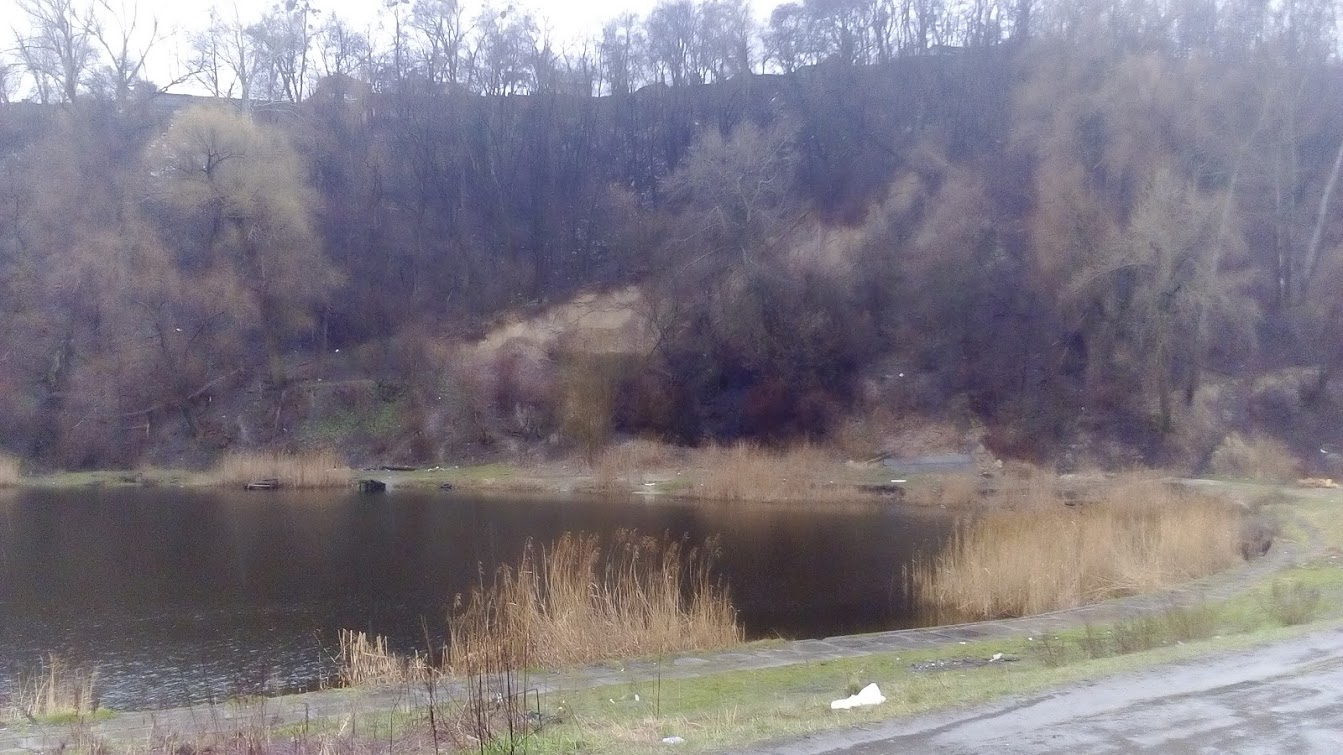
\includegraphics[width=\linewidth]{pix/DSC_0225.JPG}
%\end{center} 

%\begin{center}
%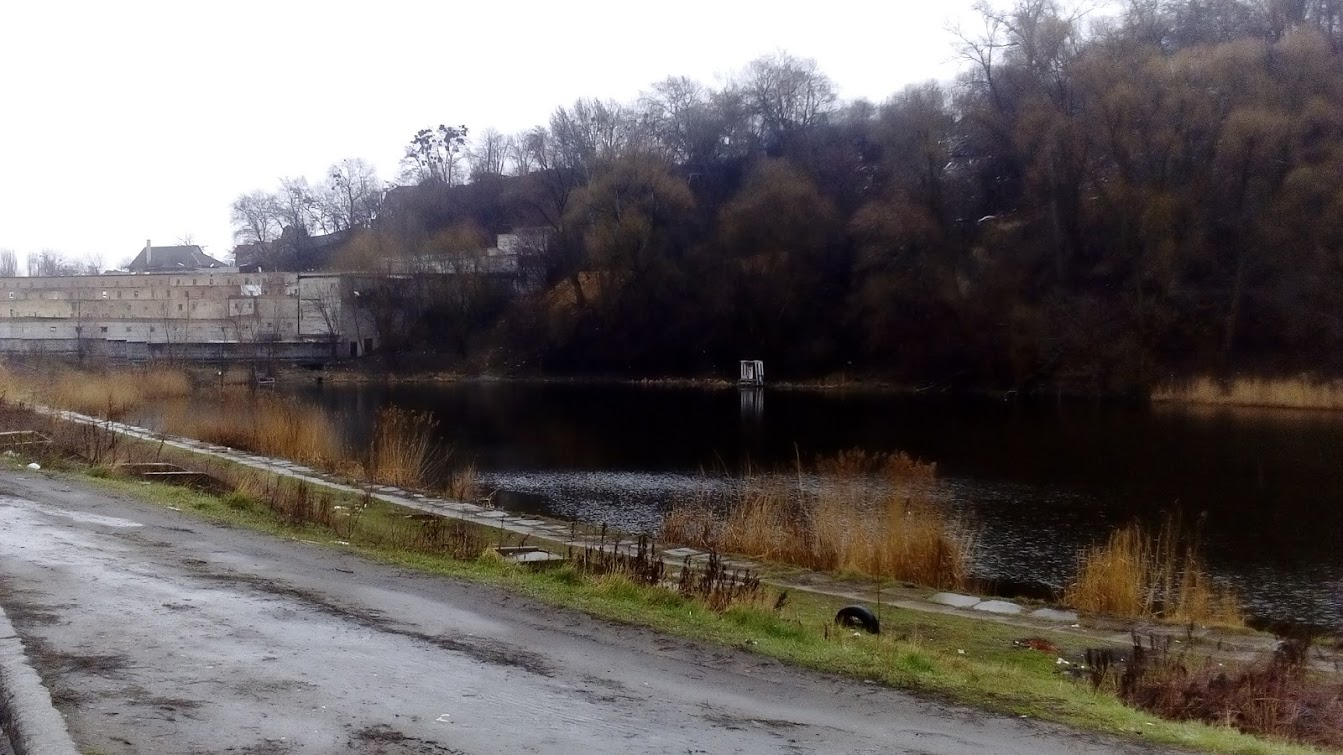
\includegraphics[width=\linewidth]{pix/DSC_0224.JPG}
%\end{center} 

%\textit{2016. Озеро в глинище на юго-запад от перекрестка Сырецкой и Копыловской. Это карьер второй половины 20 века, дореволюционные заводы кушали холм ближе к перекрестку. Фото Кати Клюевой.}
%\vspace*{\fill}
\newpage
\vspace*{\fill}
\begin{center}
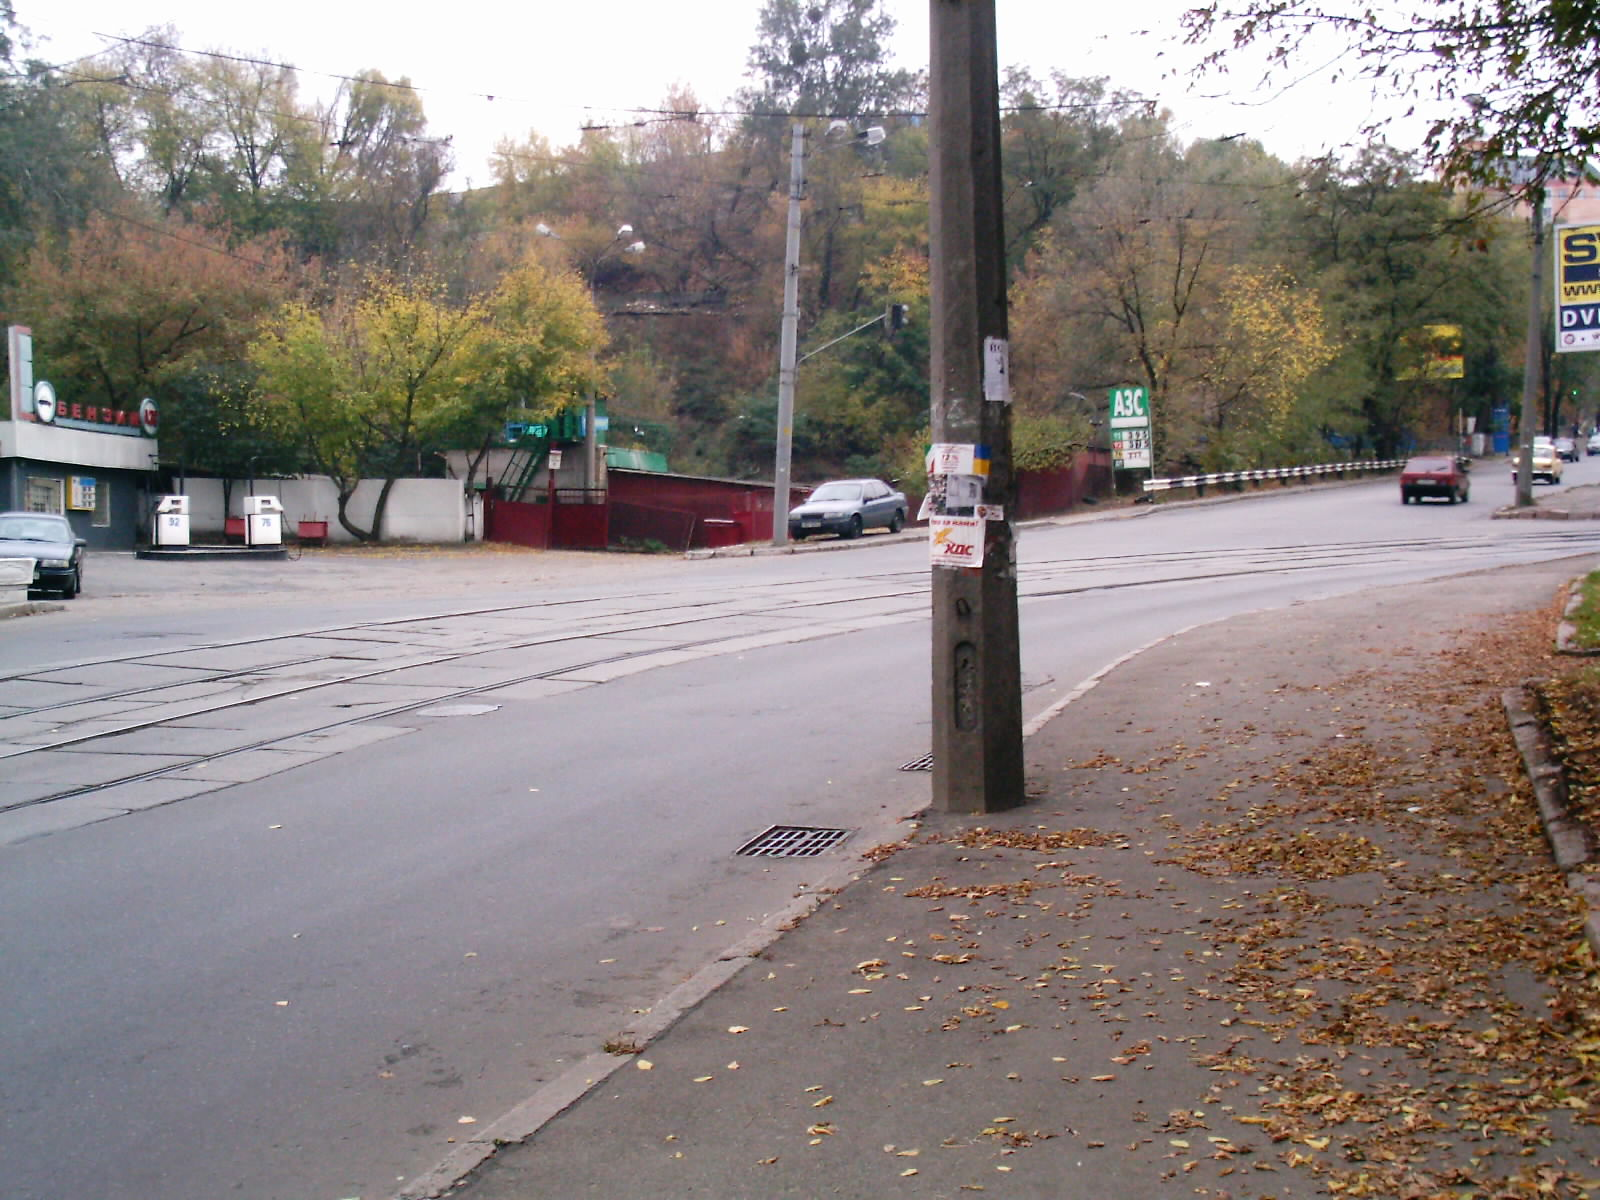
\includegraphics[width=0.90\linewidth]{pix/imag0002.jpg}

\textit{2005. Вероятно, место глинища Ясногурского.}
\end{center} 

\begin{center}
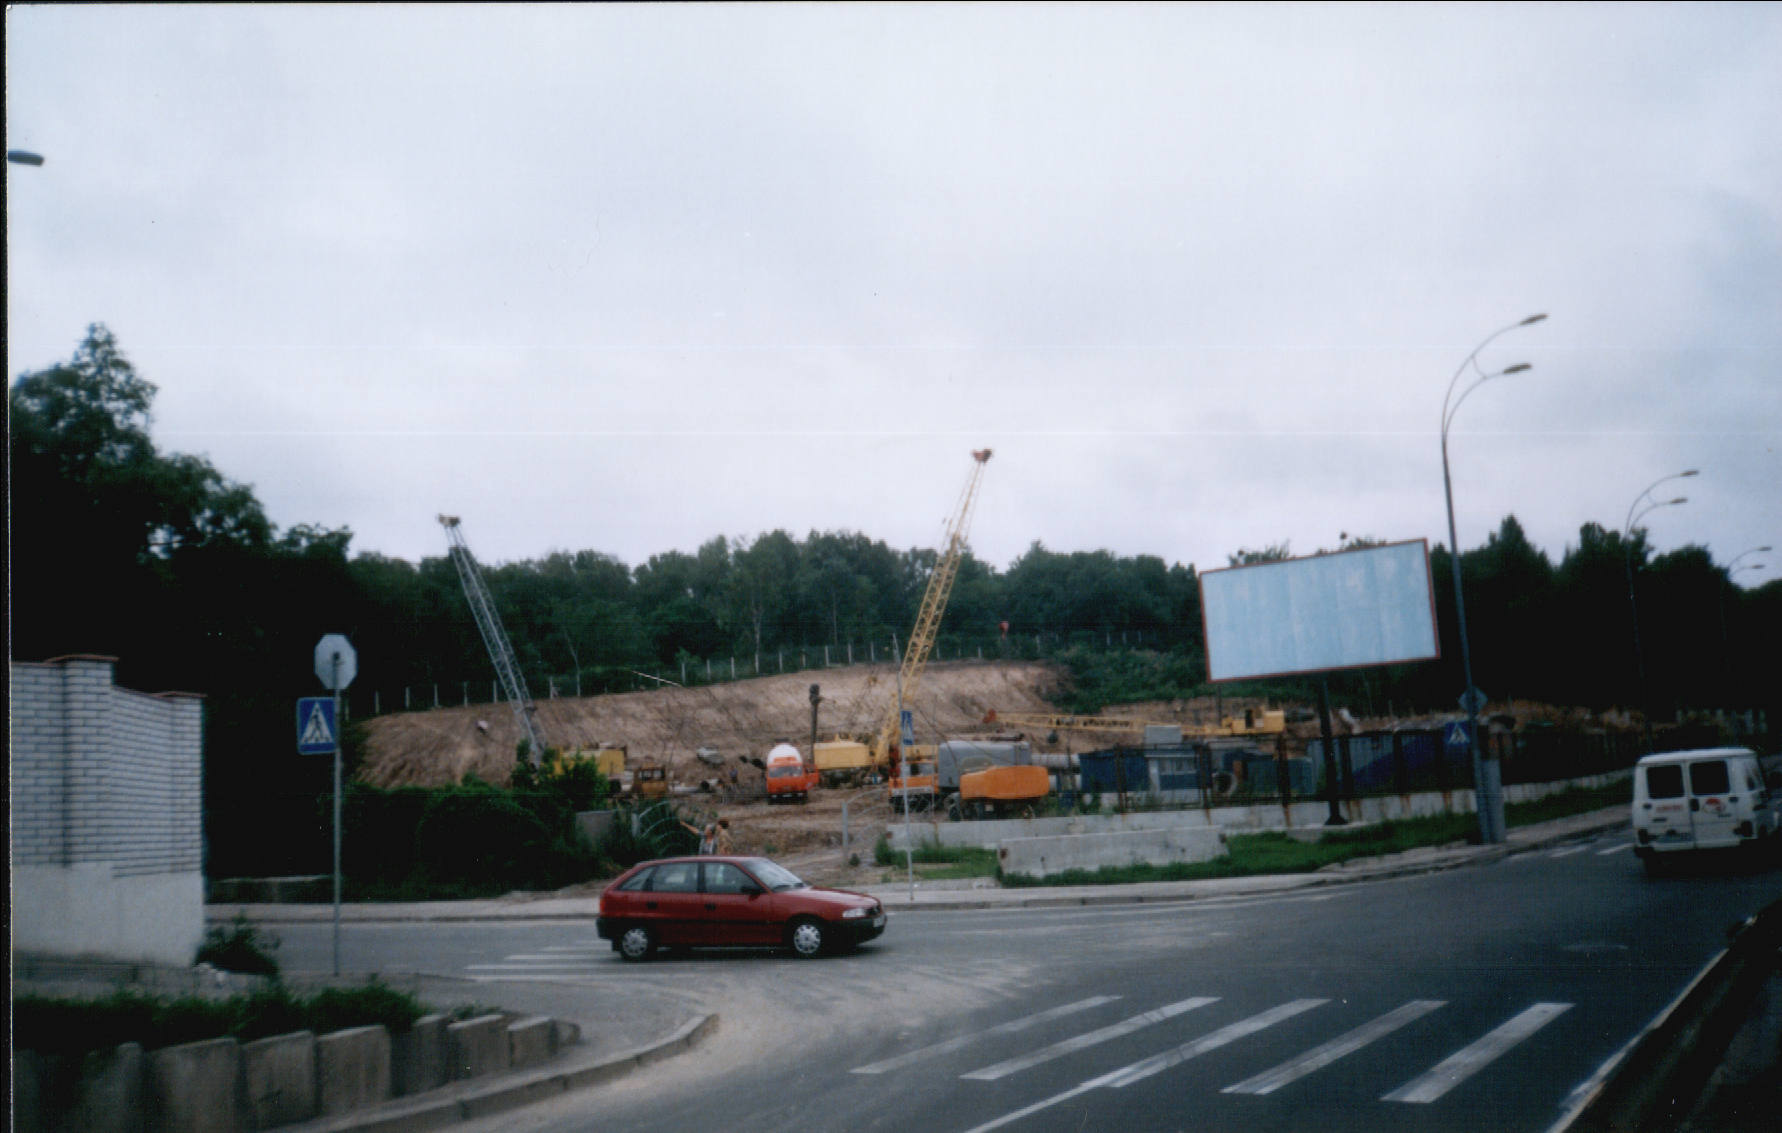
\includegraphics[width=0.90\linewidth]{pix/out0011.jpg}

\textit{2003. Застройка глинища одного из казенных заводов, южный конец Зверинецкого холма.}
\end{center} 
\vspace*{\fill}
\newpage
\vspace*{\fill}
\begin{center}
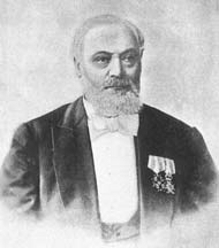
\includegraphics[width=0.60\linewidth]{faces/berner.jpg}

\textit{Бернер Яков.}
\end{center} 

\begin{center}
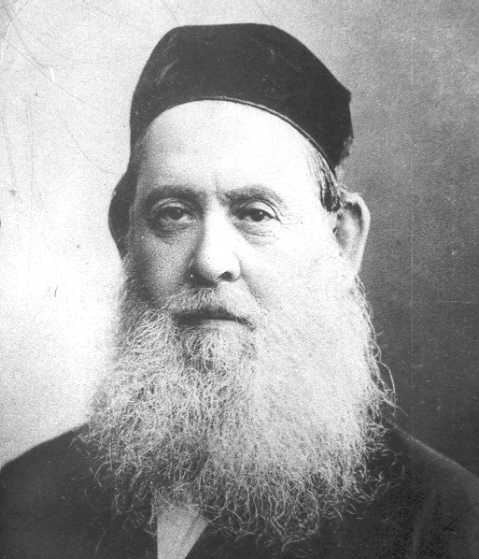
\includegraphics[width=0.60\linewidth]{faces/zajcev.jpg}

\textit{Зайцев Иона.}
\end{center} 

\vspace*{\fill}
\newpage

\begin{center}
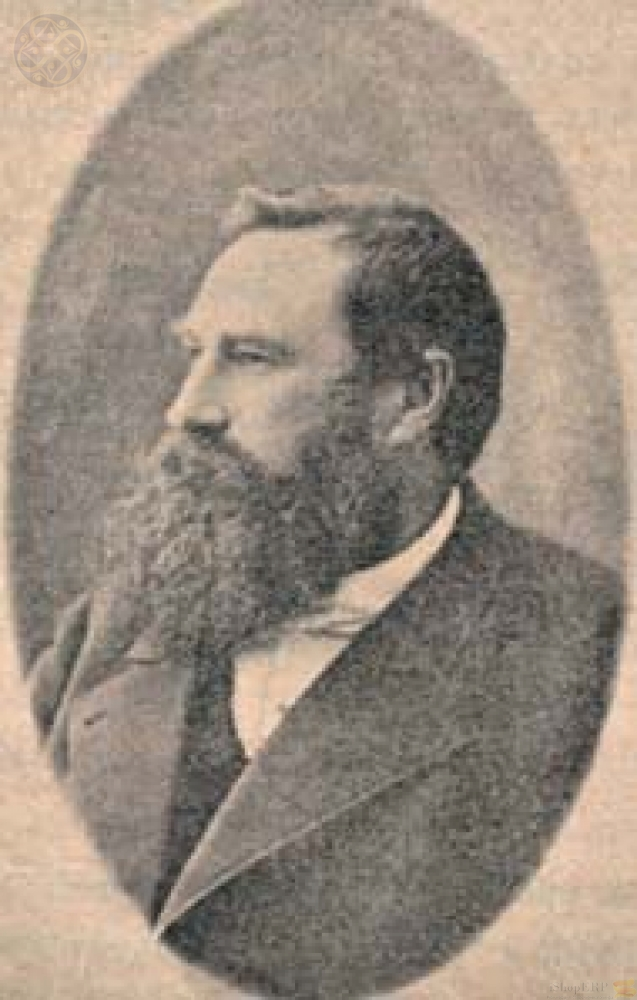
\includegraphics[width=0.50\linewidth]{faces/mihelson.jpg}

\textit{Михельсон Фридрих.}
\end{center} 

\begin{center}
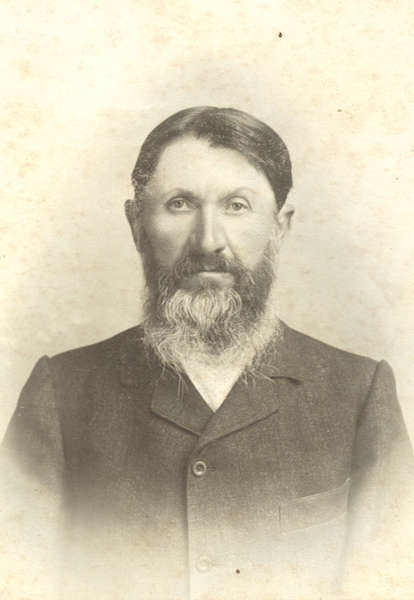
\includegraphics[width=0.50\linewidth]{faces/slepushov.jpg}

\textit{Слепушов Андрей.}
\end{center} 

\newpage
\begin{center}
\includegraphics[width=0.96\linewidth]{pix/\myimgprefix IMG_20161116_114943.jpg}


\textit{Плинфа, найденная у подножия северо-восточного мыса Зверинецкого холма, на склоне за забором ботсада примерно за остановкой «улица Выдубицкая». Окрестности известны археологам по находкам остатков гончарной слободы времен Великого Княжества Литовского и остатков здания «великокняжеского времени», которое наука отождествляет с Красным двором князя Всеволода.}
\end{center} 

\newpage

\begin{center}
\includegraphics[width=\linewidth]{pix/\myimgprefix IMG_20161116_114920.jpg}

\textit{Та же плинфа с обратной стороны.}
\end{center} 

\begin{center}
\includegraphics[width=\linewidth]{pix/\myimgprefix IMG_20161116_114743.jpg}

\textit{Другая плинфа.}
\end{center} 


\newpage


\begin{center}
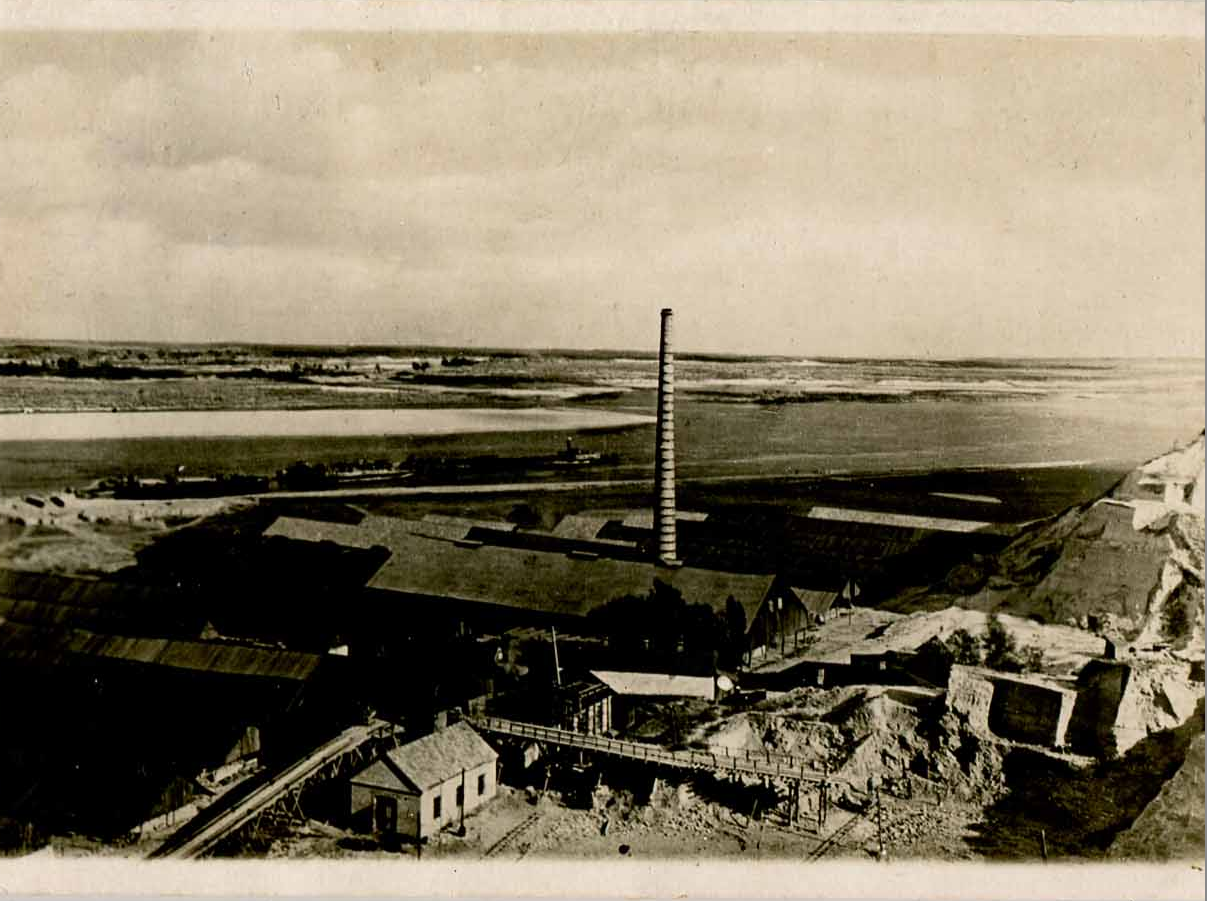
\includegraphics[width=0.95\linewidth]{pix/staiki.png}

\textit{Кирпичный завод в с. Стайки. Советская открытка.}
\end{center} 


\begin{center}
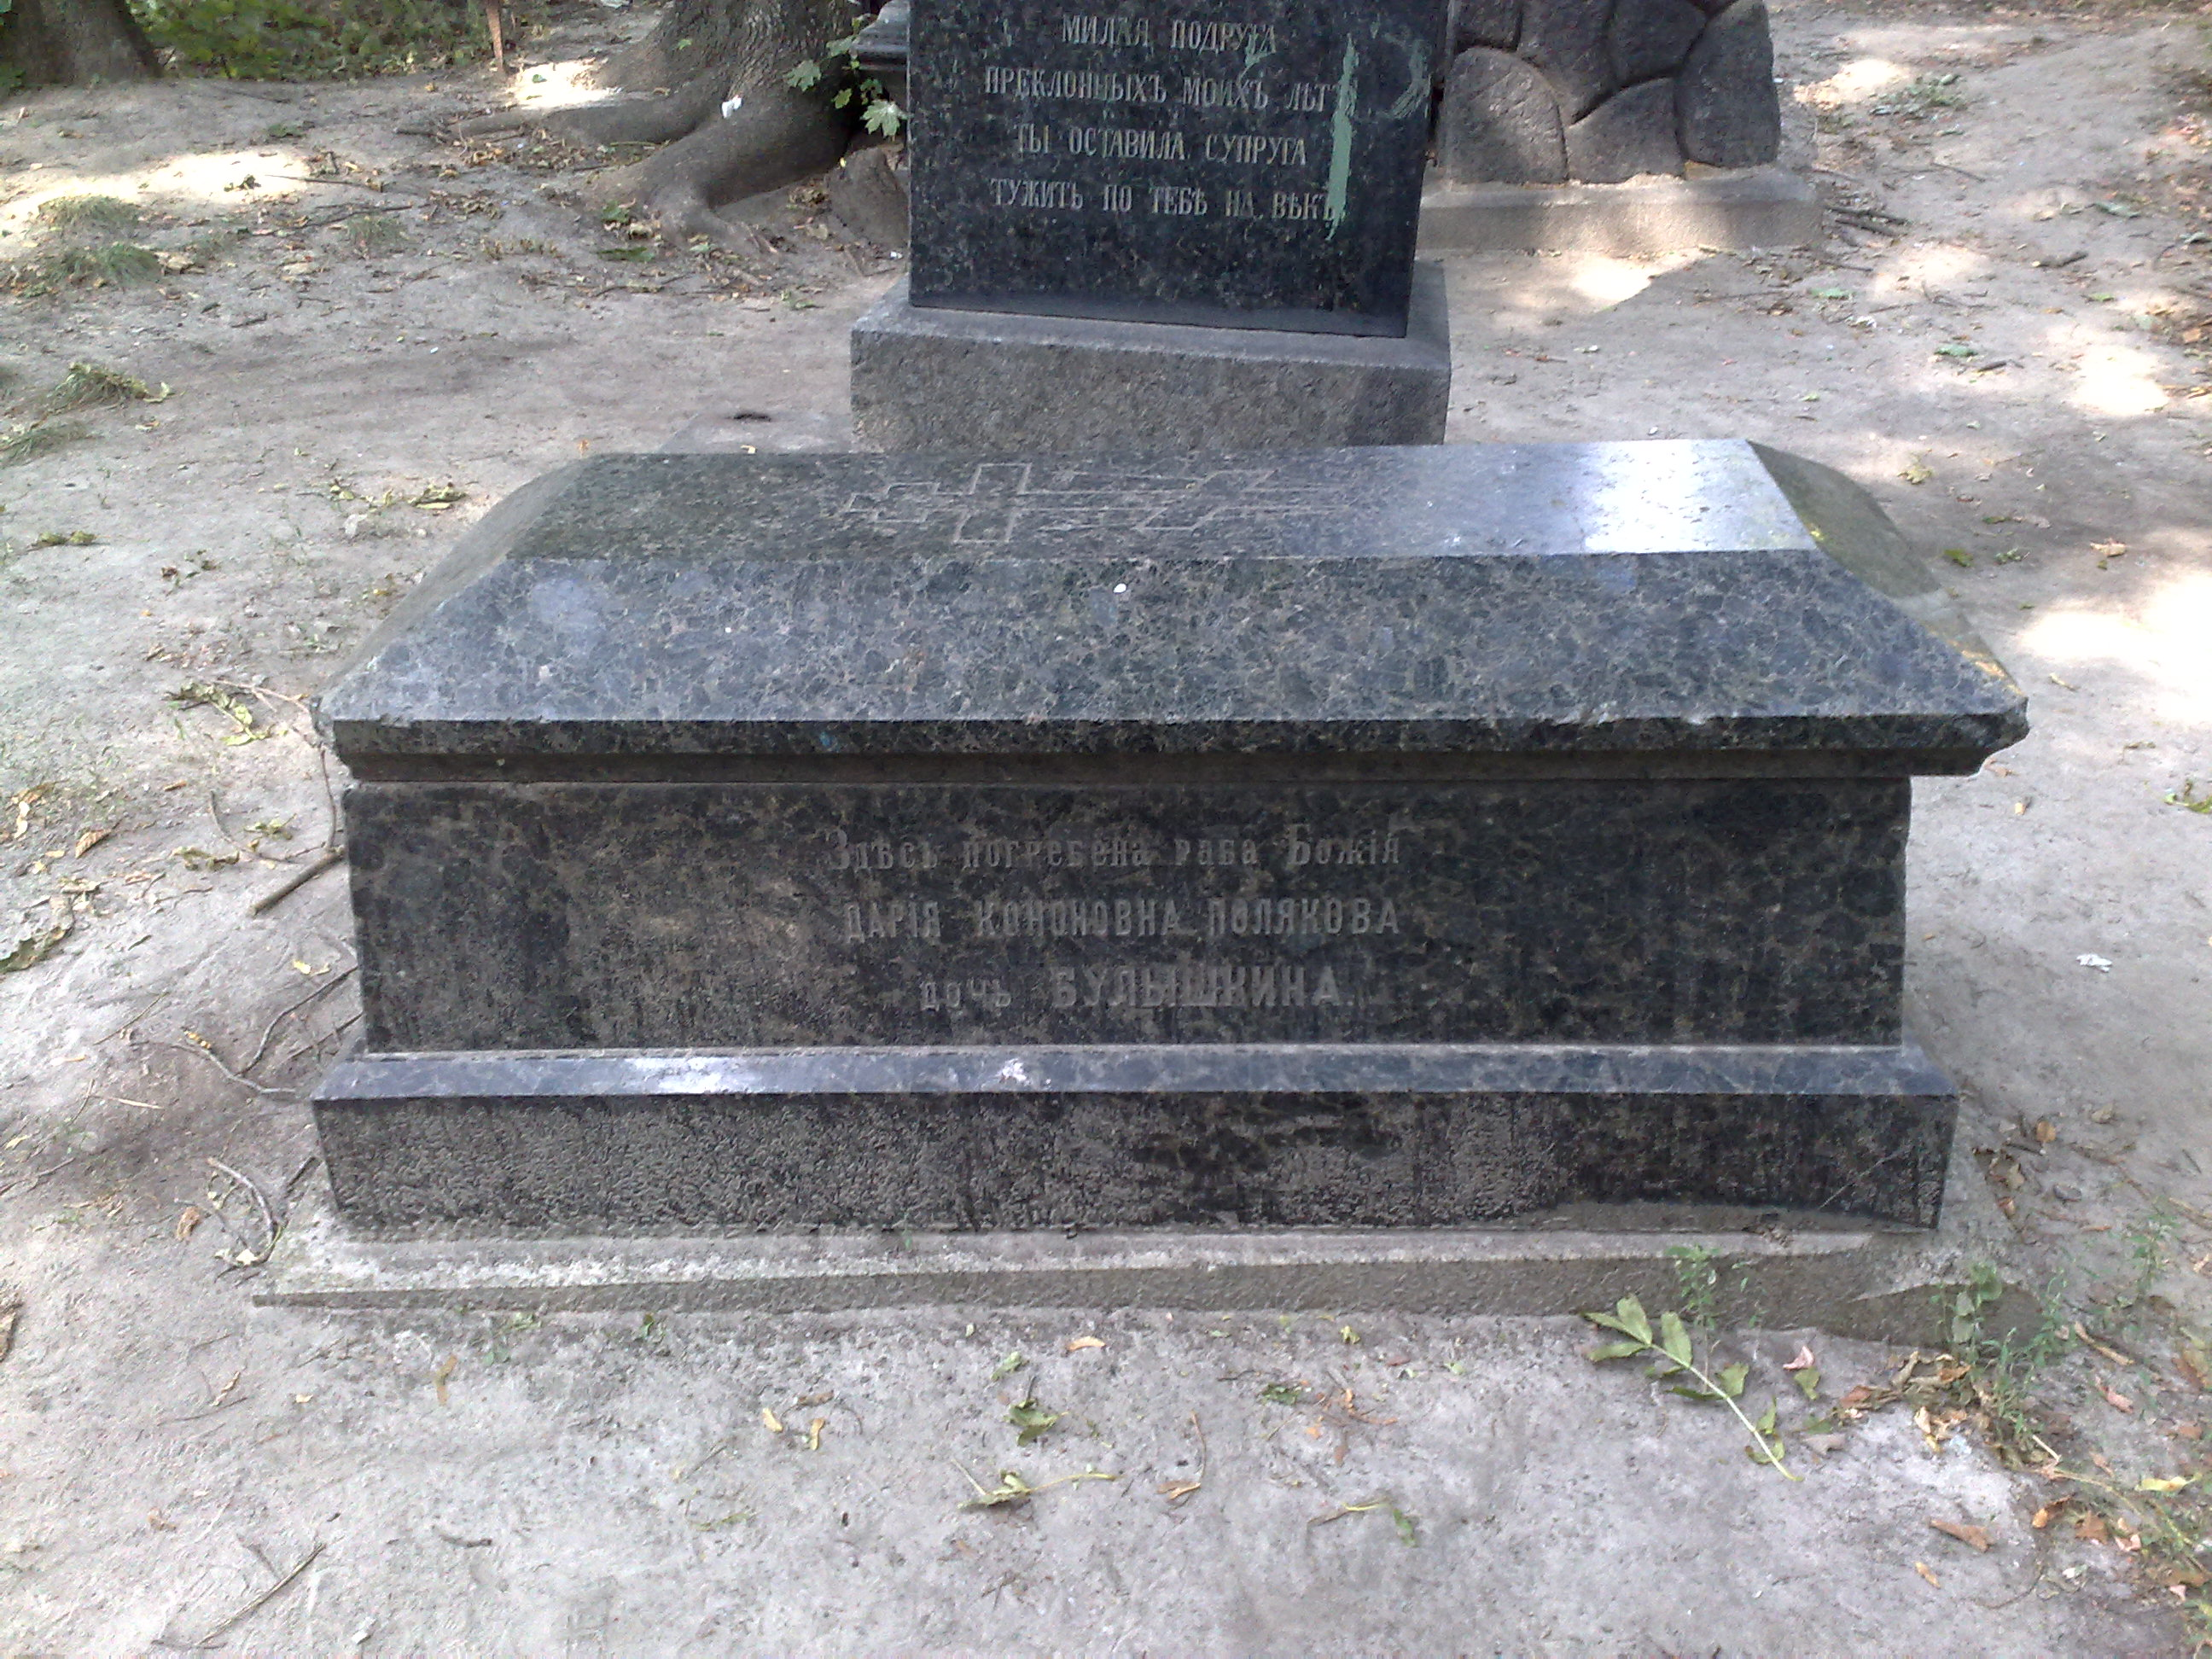
\includegraphics[width=0.95\linewidth]{pix/27082009561.jpg}

\textit{Могилы семьи Булышкиных находятся в Киеве, на старообрядческом кладбище при горе Щекавице.}
\end{center} 
